\setcounter{chapter}{13-1} %Makes the prereq chapter chapter 0

\chapter{Reinforcement Learning}

    \subsection{MDP Review}

        Last chapter, we explored MDPs, a tool for simulating a "game". We, the "player", choose which \textbf{actions} we take.
        
        \begin{itemize}
            \item Different \brow{actions} can
                \begin{itemize}
                    \item Change the \redd{state} of the world: what our system looks like.
                    \item Provide us with \purp{rewards}, based on our actions.
                \end{itemize}
        \end{itemize}

        However, we our system isn't perfectly consistent:
        
        \begin{itemize}
            \item The \gren{transitions} between states are \textbf{probabilistic}: we don't know our exact next state, but we know the \textbf{odds} of each possible next state.
        \end{itemize}

        \begin{figure}[H]
            \centering
            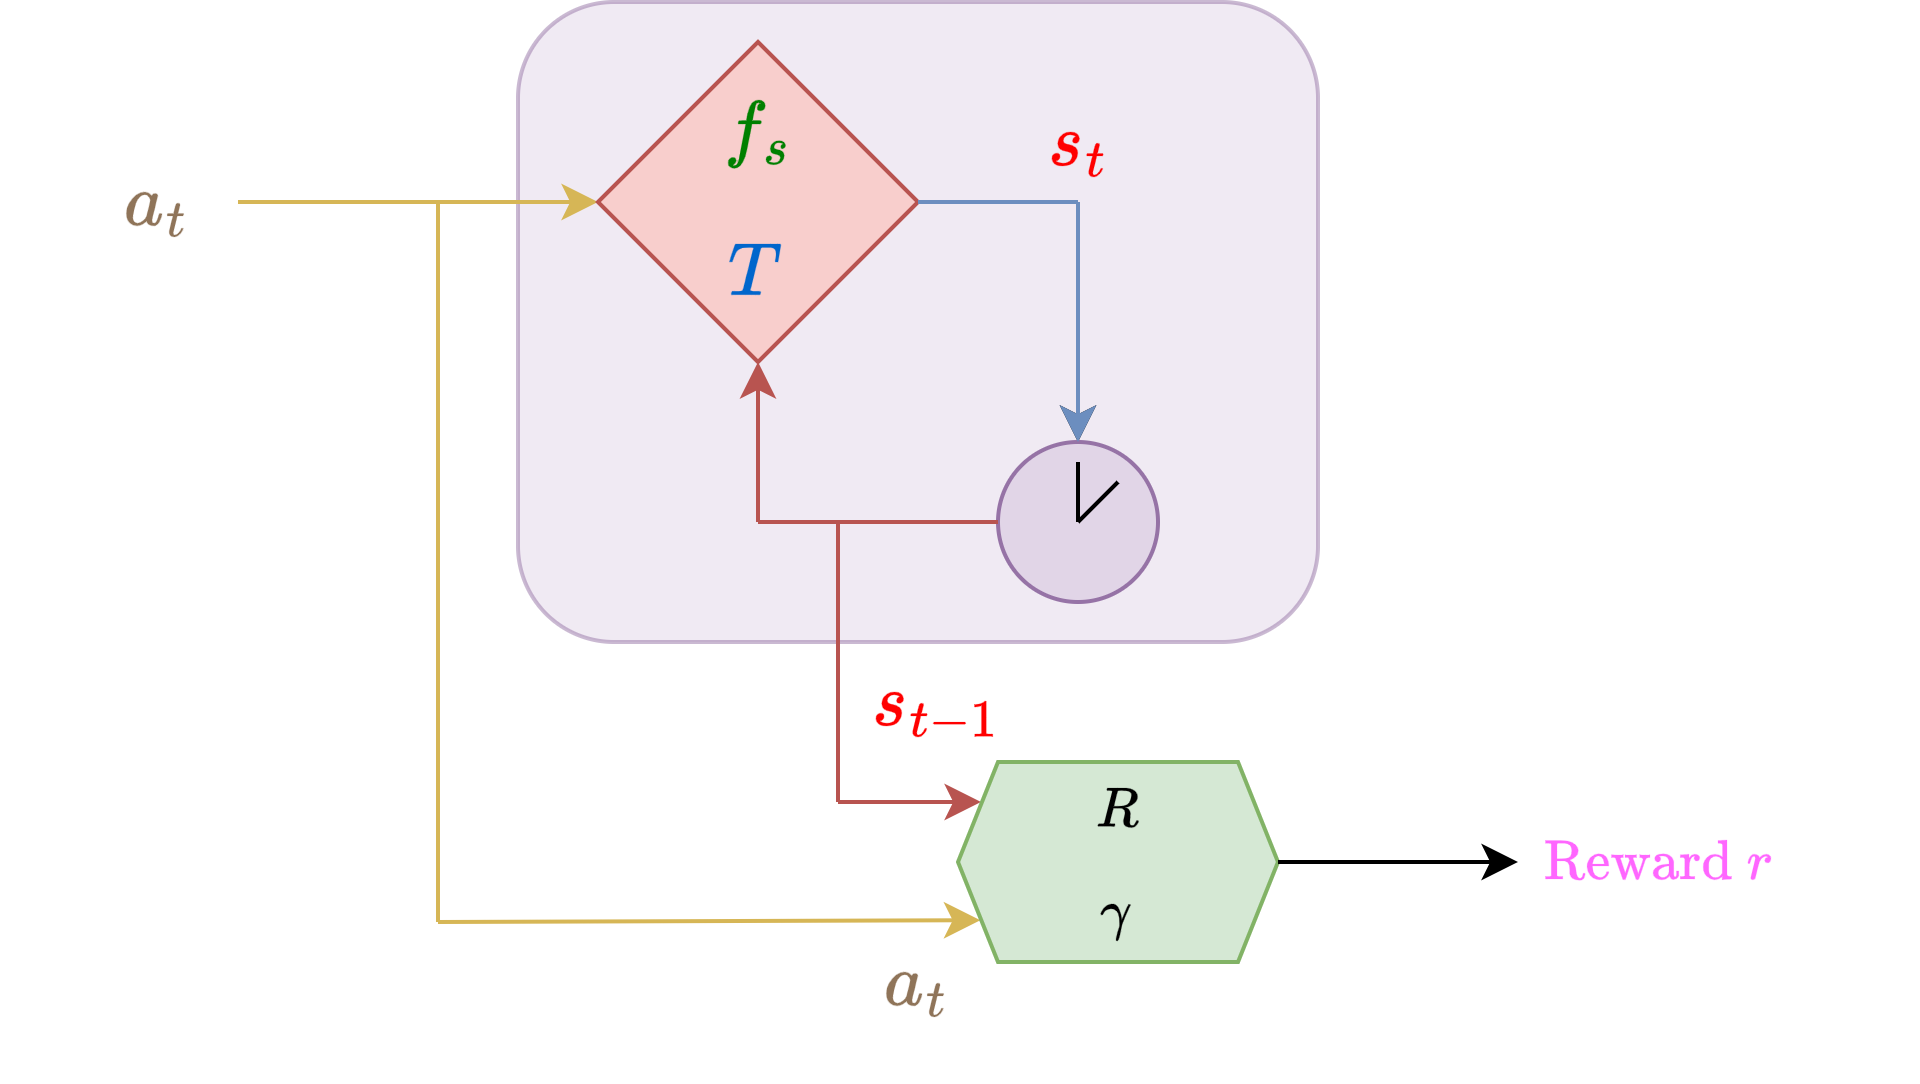
\includegraphics[width=70mm,scale=0.5]{images/mdp_images/mdp_transparent.png}
            
            \caption*{Here's our MDP: our model of a system that we can change over time.}
        \end{figure}

        Given complete knowledge of our system, we wanted to come up with the best possible strategy (\gren{policy}) for getting the most reward, over time.

        \begin{figure}[H]
            \centering
            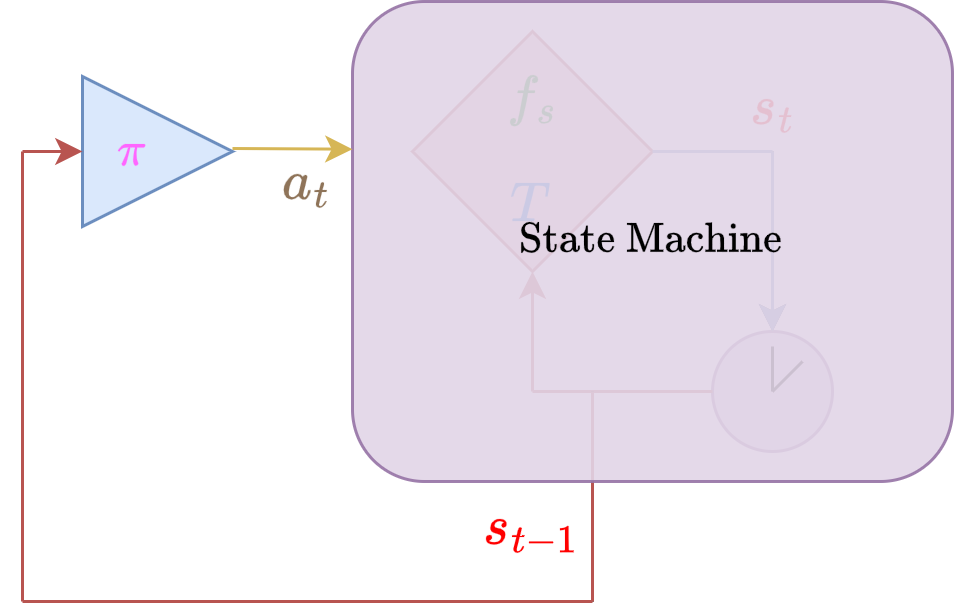
\includegraphics[width=50mm,scale=0.5]{images/mdp_images/policy_statemachine.png}
            
            \caption*{Our policy chooses different actions, based on what state our state machine gives us.}
        \end{figure}

        We evaluate our policies based on the \purp{average expected reward}, for each state.

        \begin{figure}[H]
            \centering
            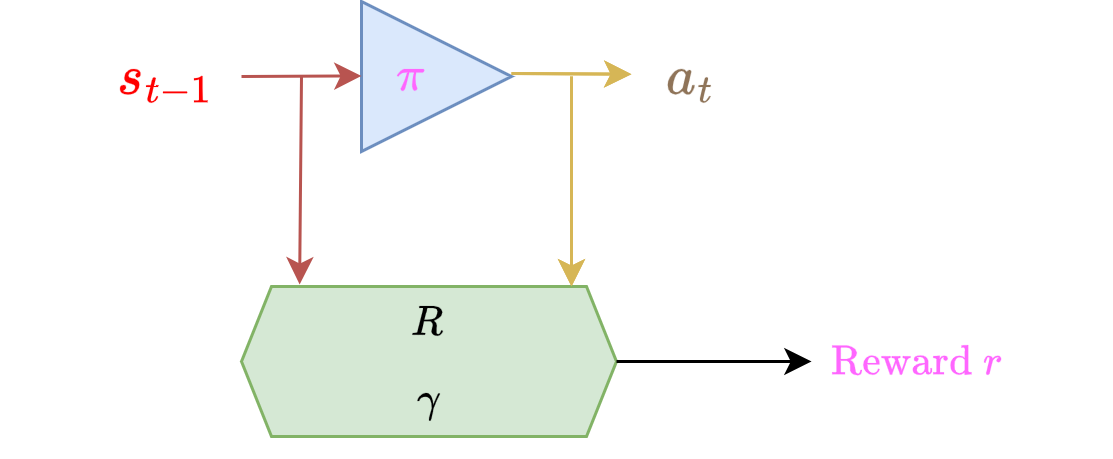
\includegraphics[width=50mm,scale=0.5]{images/mdp_images/policy_reward.png}
        \end{figure}

        Combining these three parts (state machine, reward function, policy), we would find the best policy, using \gren{value functions}, and \purp{$Q$-value functions}.



    \phantom{}

    \subsection{What if we don't know as much?}

        There's a major limitation of this approach:

        \begin{itemize}
            \item It assumes we have know everything about our system.\\
        \end{itemize}

        \begin{concept}
            \vocab{Value functions} can only be computed if you have \orgg{complete knowledge} of your MDP:

            \begin{itemize}
                \item What are the odds of your \gren{state transitions}?
                \item What \purp{rewards} will you get in different situations?
            \end{itemize}

            Without this information, it's not possible to compute the "value" of a policy, using our previous techniques.
        \end{concept}

        \begin{equation}
            V_{\grn{\pi}}^{\pur{H}}\big(\red{s} \big) \;\;=\;\; 
                \pur{R} \Big( \red{s},\grn{\pi}\big(\red{s}\big) \Big) +
            \sum_{\blu{s'}}  
                    \;\;
                    \grn{T} \Big(          \red{s},\grn{\pi}\big(\red{s}\big),\blu{s'} \Big)
                    \;\cdot\; 
                    V_{\grn{\pi}}^{\pur{H-1}}\big(\blu{s'} \big)
        \end{equation}

        \begin{itemize}
            \item This equation is impossible to compute without those crucial variables $T$ and $R$.

            \item But in plenty of real situations, you won't know exactly what effects your actions might have.
        \end{itemize}

        \begin{figure}[H]
            \centering
            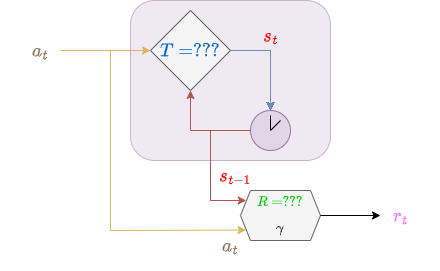
\includegraphics[width=70mm,scale=0.5]{images/rl_images/mdp_unknown.png}   
            \caption*{Often, we don't know $T$ and $R$.}
        \end{figure}



    \phantom{}

    \subsection{Learning about our MDP}

        If we don't know our transitions, or our rewards, our model is reduced to a simple box: based on an action, you see the next state $s_t$, and your reward $r_t$.
            \note{This simplified object is called the "environment" for our player.}

        \begin{figure}[H]
            \centering
            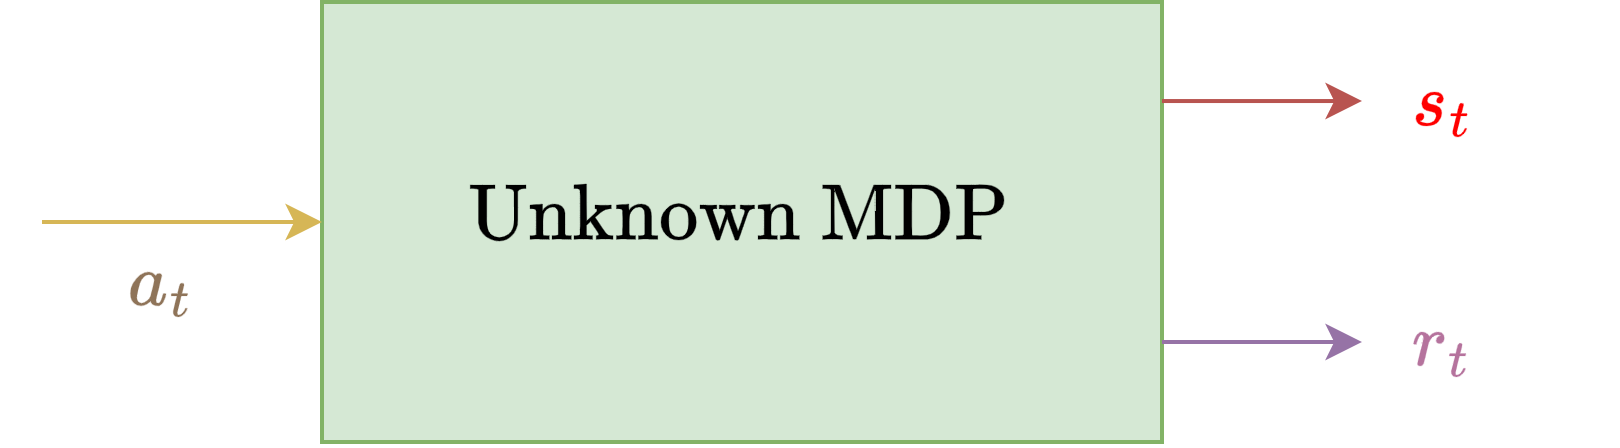
\includegraphics[width=50mm,scale=0.5]{images/rl_images/mdp_blackbox.png}
            \caption*{Since we don't know what's inside, we reduce our MDP to a simple input-output machine.}
        \end{figure}
        
        
        The only way to learn our MDP is to \purp{exploring} and gathering data.

        The only way we can interact with our MDP is by taking \brow{actions}. So, we do that:

        \begin{itemize}
            \item We are given the initial state $\red{s_0}$.
            \item We experiment, and take an action $\bro{a_1}$.
            \item We learn some information:
                \begin{itemize}
                    \item We get reward $\pur{r_1}$.
                    \item We transition to new state $\blu{s_1}$.
                \end{itemize}
        \end{itemize}

        Repeat.

        \subsecdiv

        We continue until we're satisfied, choosing actions and getting feedback.\\

        \begin{concept}
            In \vocab{reinforcement learning} (RL), we want to learn more about our MDP, so we \purp{experiment}, by taking different \brow{actions}.

            \begin{itemize}
                \item We take an \brow{action}, and see what it \redd{does} (state transition, reward).
                \item We do it again. And again.
                
            \end{itemize}

            By \gren{experimenting}, and continuously getting feedback, we slowly learn about our MDP. This gathers up our data:

            \begin{equation*}
                \begin{bmatrix}
                    s_0 & s_1 & s_2 & \cdots s_{n}
                \end{bmatrix}
                \qquad
                \begin{bmatrix}
                    r_1 & r_2 & \cdots r_n
                \end{bmatrix}
            \end{equation*}
        \end{concept}

        \miniex You have a panel of buttons. You ask yourself, "what does this one do?", and press one of them.

        \begin{itemize}
            \item Then, you might ask: what if I press them in a different order? In different situations?
            \item As you learn more, you gradually figure out a "better" way to play.
        \end{itemize}

        \subsecdiv 

        This is very similar to how you might play a video game when you first pick it up.




        \phantom{}

    \subsection{Reinforcement Learning}

        Now that we know what to do, we need to \textbf{formalize} it.
            \note{Represent things with math, give each part a name, etc. Things that will make it easier to talk about.}

        We can divide up this process into two:\\

        \begin{definition}
            Our \vocab{reinforcement learning} (RL) problem can be divide into two main parts:

            \begin{itemize}
                \item The \vocab{learner}: this is the "player" of the game. 
                    \begin{itemize}
                        \item The learner chooses which \brow{actions} to take: they decide the policy.

                        \item Based on what they observe from the environment, they learn to make \orgg{different choices}.

                        \item Eventually, the learner's goal is to make better choices, to get the most \purp{rewards}.
                    \end{itemize}

                \phantom{}

                \item The \vocab{environment}: this is the "game" that the player is interacting with.

                    \begin{itemize}
                        \item The environment reacts to the learner's actions, responding with a \purp{reward} and \redd{state change}.
                    \end{itemize}
            \end{itemize}

            The learner is trying to \gren{learn} about the environment, and discover the best \gren{policy}.
        \end{definition}

            \note{"Learning a better policy" is what we wanted in the MDP chapter: this time, it just takes more work.}
        
        The learner chooses the action, and the environment teaches the learner. So, they work in a feedback cycle:
            \note{Why does our diagram use $s_{t-1}$ and $r_{t-1}$? Because \purp{past} data is used to make \gren{future} decisions, like $a_t$.}

        \begin{figure}[H]
            \centering
            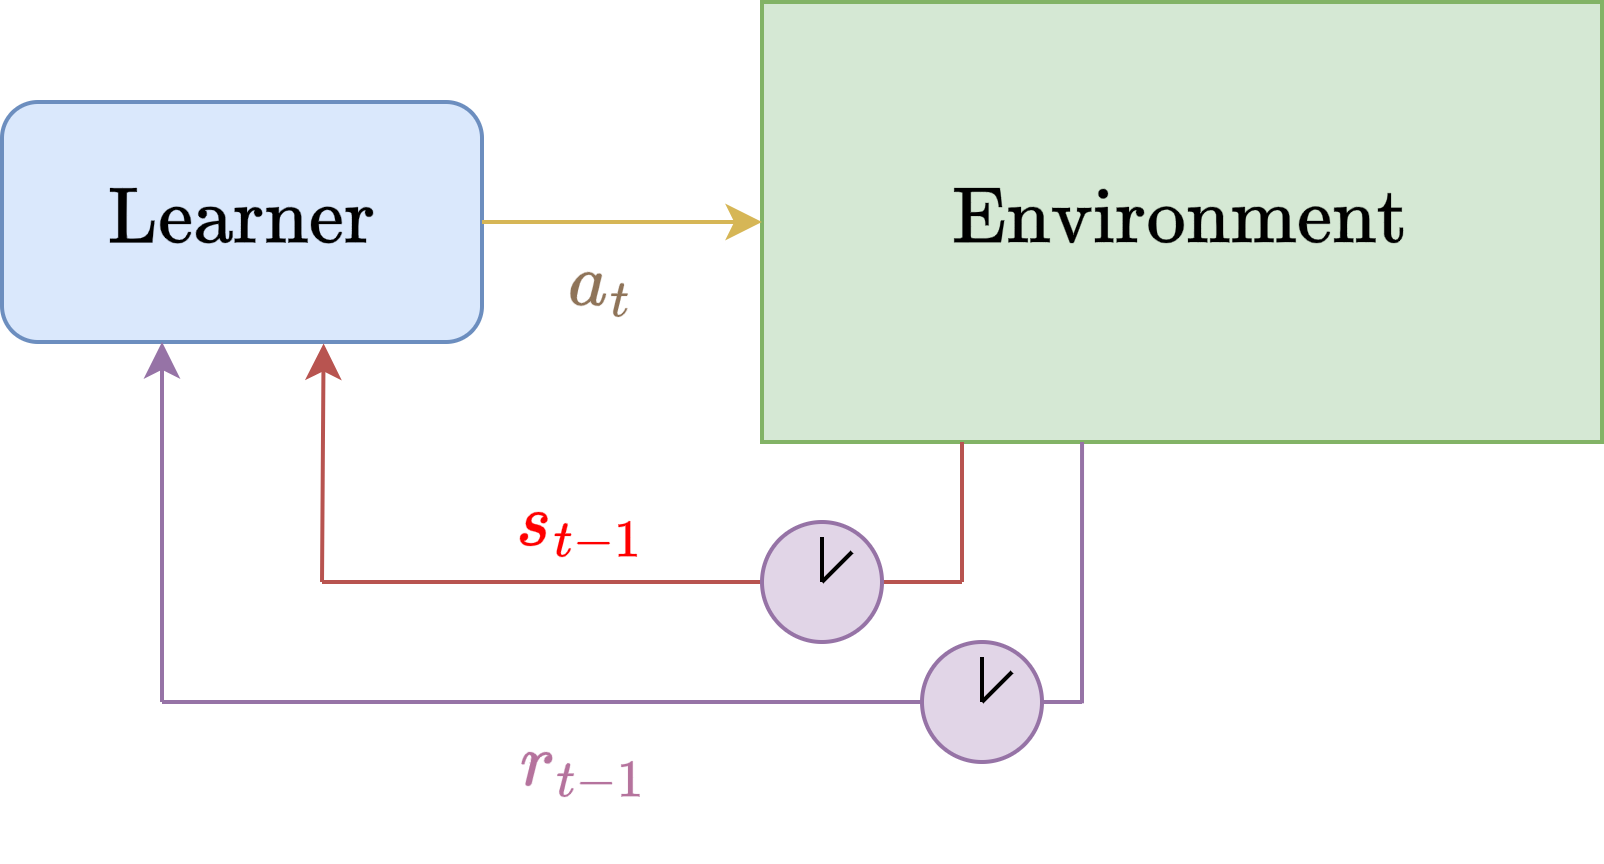
\includegraphics[width=50mm,scale=0.5]{images/rl_images/learner_environment.png}
            \caption*{Our learner makes decisions, while the environment gives feedback on those decisions. This feedback is used in the future to make better decisions.}
        \end{figure}

        \begin{notation}
            In this chapter, we use capital $R$ to represent the reward \purp{function}, and lower-case $r_t$ to represent a \gren{single} reward at time $t$.

            \begin{equation*}
                R \big( \red{s_{t-1}},\bro{a_t} \big) =\pur{r_t}
            \end{equation*}
        \end{notation}

        

        If we expect our environment to behave like an MDP, that's what we'd put inside the "environment" block. But, RL isn't necessarily limited to that framework:\\


        \begin{clarification}
            So far, we've used MDPs as a concrete example for RL, but RL can be used for some other related systems, as well.
        \end{clarification}

        \miniex One alternative environment is the "partially observable (PO) MDP". 
            \note{This requires more inference than we'll cover in this class.}




    \phantom{}

    \subsection{Supervised vs. Unsupervised vs. RL}

        RL is a bit different from our previous training frameworks: "supervised" and "unsupervised".

        Let's review:

        \begin{itemize}
            \item \vocab{Supervised learning}: you're explicitly given an input $\ex{x}{i}$, and a desired output $\ex{y}{i}$
                \begin{itemize}
                    \item \miniex This is similar to being given a test, with the answer key.
                \end{itemize}
            \item \vocab{Unsupervised learning}: you're given inputs, but you're not given an output: you have to look for patterns or structure without outside help.
                \begin{itemize}
                    \item \miniex You're given a set of photos, and asked to sort them, based on what object is in the image. You aren't given labels.
                \end{itemize}

            \item \vocab{Semi-supervised learning}: you're given \textit{some} answers, but not most of them.
        \end{itemize}

        Reinforcement learning is a bit different:\\

        \begin{concept}
            \vocab{Reinforcement learning} (RL) provides data to the model differently from supervised / unsupervised frameworks:

            \begin{itemize}
                \item The model has some \purp{choice} in which data it sees: it chooses \brow{action} $a_t$, which affects the feedback $s_t$ and $r_t$.

                \item This means the model doesn't just learn by observing the data: it \gren{interacts} with it.
            \end{itemize}

            Over the course of training, our model can make \orgg{different choices} about what to learn, based on what it's already seen.
        \end{concept}

        This approach forces our model to not only learn the structure of the data, but how to ask questions.
            \note{Just like how a student learns when to ask questions, and what they need to practice.}
        

        

    \pagebreak

\section{Reinforcement Learning Algorithms Overview}

    Our "learner" is more complex than our previous system for choosing actions:

    \begin{itemize}
        \item It gradually \gren{learns} the rewards and state transitions.
        \item It has to not only choose the best rewards, but also choose what parts of the environment to \purp{explore}.
    \end{itemize}

    But even so, it only really makes one decision: choosing actions. It's still a type of \gren{policy}.\\

    \begin{concept}
        A \vocab{reinforcement-learning (RL) algorithm} is a type of \gren{policy}.

        It chooses our \brow{next action} based on all of its past data:

        \begin{itemize}
            \item States, actions, rewards
        \end{itemize}

        \subsecdiv

        Similar to $\pi(s)$, the goal is to \purp{maximize rewards}.

        \begin{itemize}
            \item However, our RL algorithm first has to \orgg{explore} different parts of the environment, to know what the rewards and transitions are.
            \item This is why it needs to use all of our past data: to \gren{learn}.
        \end{itemize}
    \end{concept}

    When we're finished training, it may be possible to just keep the policy $\pi: \mathcal{S} \to \mathcal{A}$, and discard all of our past data.
        \note{This is similar to how, when we finish training our NN, we just give people the model, not the training data.

        \phantom{}

        Our trained model contains the information we need to make decisions: we don't need all the training data.}


    

    \phantom{}

    \subsection{Evaluating RL algorithms}

        How do we evaluate our RL algorithm? There are a couple different ways:\\

        \begin{concept}
            We can \vocab{evaluate} our learning algorithm based on \gren{how long} it takes for it to learn a mostly-\purp{optimal policy}.

            \begin{itemize}
                \item In other words: "how long does it take to train?"
            \end{itemize}

            In this scenario, we ignore the rewards we get while learning: our model is allowed to make \orgg{mistakes}.
        \end{concept}

        In other situations, we want our model to do well while training:\\

        \begin{concept}
            We can also \vocab{evaluate} our learning algorithm based on \purp{expected rewards} while training.

            \begin{itemize}
                \item In other words, "can it perform well, while still training?"
            \end{itemize}

            In this scenario we're focused on rewards \orgg{while learning}: we don't want our model to make as many mistakes.
        \end{concept}

        Which do we usually use?

        \begin{itemize}
            \item We use the first one more \gren{often}, because it's often easier to design and measure: we just train the model first, and keep track of the total time.

            \item The second one is more \purp{challenging}: it's difficult to create a model that can perform reasonably well, while still learning.
                
        \end{itemize}

        But, sometimes the latter is necessary: you may need to train in real situations, where the rewards really matter.\\

        \begin{concept}
            If we have a \purp{safe}, cheap environment to train in, it's easier to train first, and then figure out performance later.

            But if you're training in a \gren{costly} environment, you need to make sure your model performs well, even while still training.
        \end{concept}

        \miniex Suppose that you want to train a car in real traffic environments: simulations aren't good enough.

        \begin{itemize}
            \item You really don't want your car to make major mistakes in real traffic: even if you're "training", the accidents are very real.
        \end{itemize}



        \phantom{}

    \subsection{Different types of RL models}

        In a reinforcement learning situation, what we're missing is \gren{information} about our model. 

        \begin{itemize}
            \item We don't know our transitions $T$, or our reward function $R$.
            \item In our value-iteration setting, we used these to compute what's \orgg{optimal}: $Q$ and $\pi$.
        \end{itemize}

        Value iteration can use \gren{full information}:

        \begin{figure}[H]
            \centering
            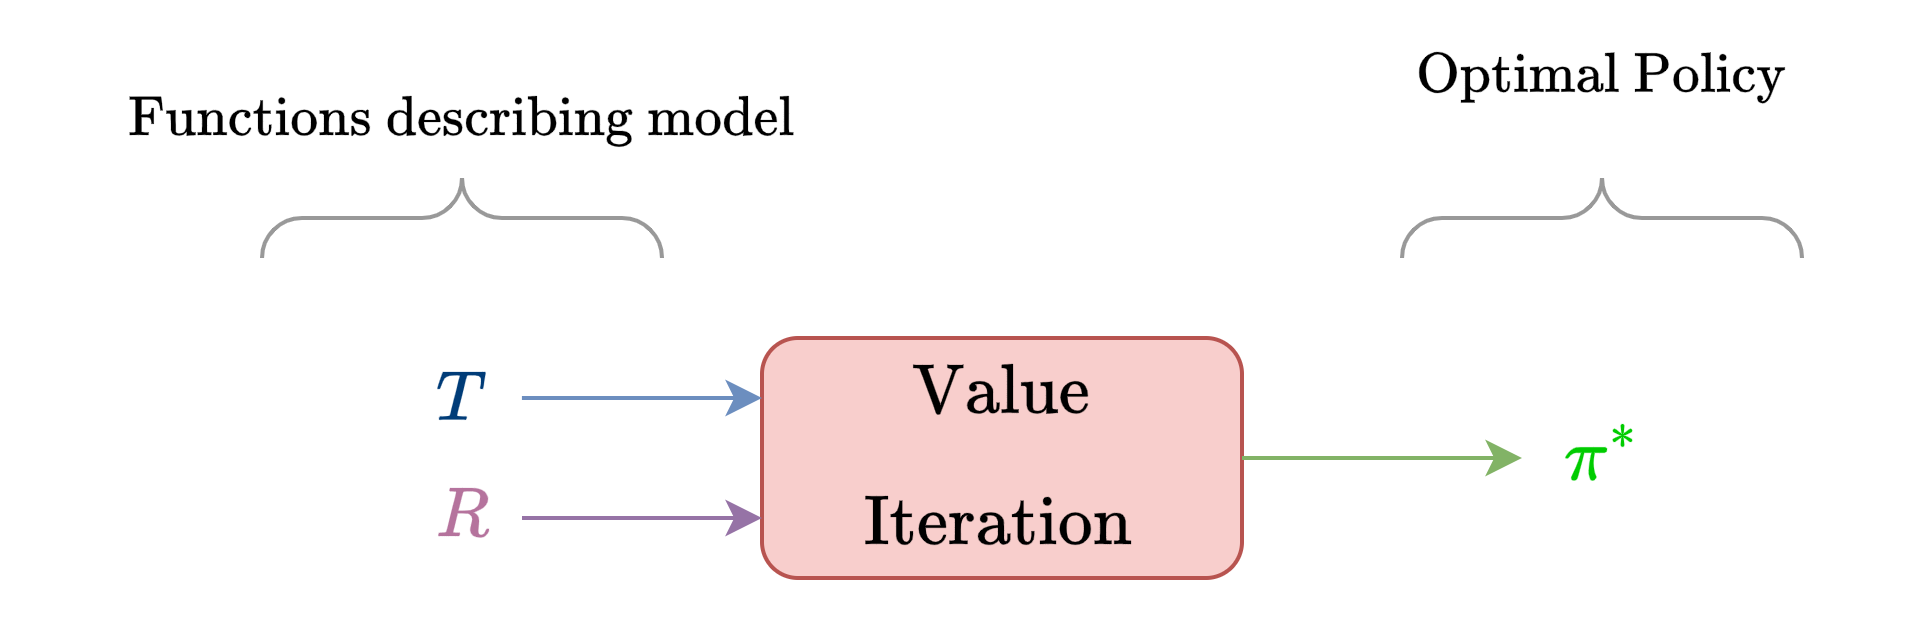
\includegraphics[width=90mm,scale=0.5]{images/rl_images/value_iteration.png}
        \end{figure}

        Reinforcement learning is more restricted. We have \purp{limited data}: some data points $s_t$ and $r_t$.
        
        \begin{figure}[H]
            \centering
            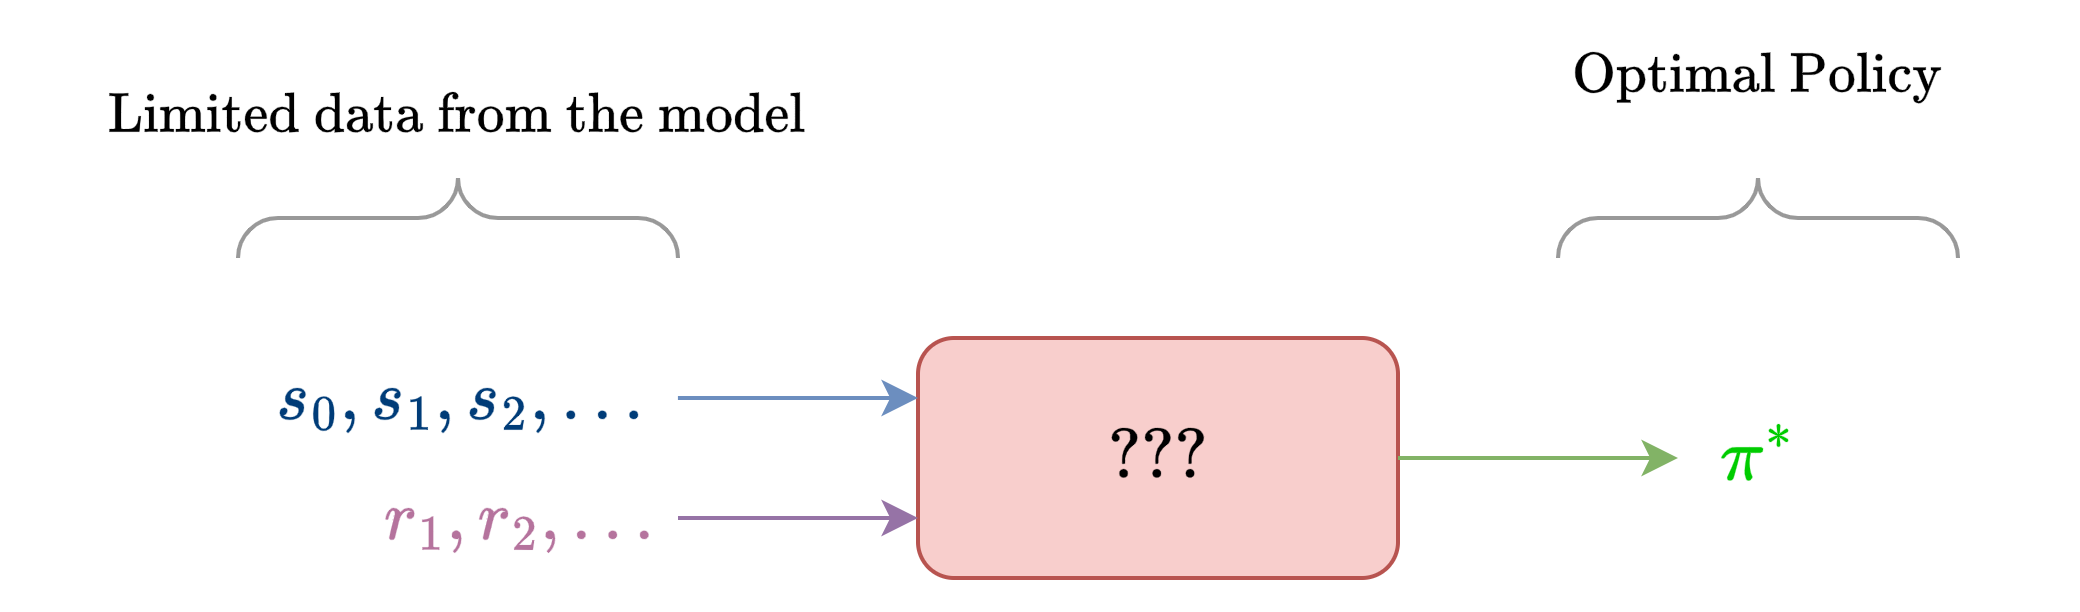
\includegraphics[width=90mm,scale=0.5]{images/rl_images/reinforcement_learning_unknown.png}
        \end{figure}





    \subsection{Types of Reinforcement Learning}

        There are multiple ways we can solve this problem. We'll focus on two types of approaches: \purp{model-based} and \gren{model-free} methods.

        In a \purp{model-based} RL algorithm, we use our data to try to \orgg{guess} the MDP model: we compute an approximation of $T$ and $R$.

        \begin{itemize}
            \item Once we've computed $T$ and $R$, we can use \textbf{value iteration}.
        \end{itemize}

        \begin{figure}[H]
            \centering
            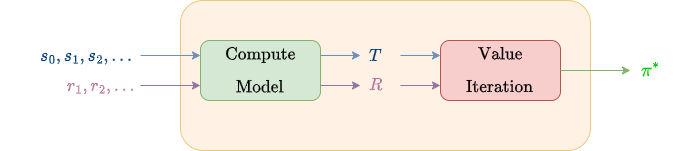
\includegraphics[width=90mm,scale=0.5]{images/rl_images/model_based.png}
            \caption*{In this approach, we can re-use our previous logic.}
        \end{figure}

        \begin{definition}
            A \vocab{model-based} RL algorithm uses our previous MDP techniques to the find the \textbf{optimal policy}. This approach requires \orgg{knowledge} of our model.

            \begin{itemize}
                \item First, we \purp{approximate} our \gren{model} ($T$ and $R$) based on data ($s_t$ and $r_t$).
                \item Then, we use that to do \orgg{value iteration}.
            \end{itemize}
        \end{definition}

        Our other approach is to use a \gren{model-free} RL algorithm, where \orgg{skip} trying to compute $T$ and $R$.
        
            \begin{itemize}
                \item Instead, we \purp{directly} compute either $Q$ or $\pi^*$.
                    \note{We don't even bother learning our MDP.}
            \end{itemize}

        \begin{figure}[H]
            \centering
            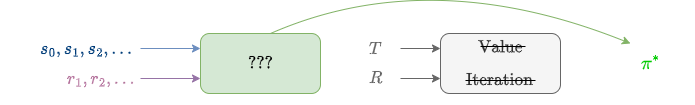
\includegraphics[width=90mm,scale=0.5]{images/rl_images/model_free.png}
            \caption*{We don't need $T$, $R$, or value iteration.}
        \end{figure}

        \begin{definition}
            A \vocab{model-free} RL algorithm gives up our previous MDP techniques. Meaning, we \orgg{don't try} to directly compute our model ($T$ and $R$).

            Instead, we find other ways to use our data ($s_t$ and $r_t$):

            \begin{itemize}
                \item In \vocab{Q-learning}, we approximate the \purp{state-action value function} $Q(s,a)$, using \gren{$Q$-learning}.
                    \begin{itemize}
                        \item We find the best policy by maximizing $Q(s,a)$.
                    \end{itemize}

                \item In \vocab{policy search}, we represent our policy $\pi$ with a \purp{computable function} $f(\theta)$, and try to \gren{optimize} that function.
                    \begin{itemize}
                        \item We might use gradient descent, for example.
                    \end{itemize}
            \end{itemize}
        \end{definition}

        In this chapter, we will go in the following order:

        \begin{itemize}
            \item Model-free methods
                \begin{itemize}
                    \item $Q$-learning
                    \item Policy Search
                \end{itemize}
            \item Model-based methods
            \item Bandit problems
        \end{itemize}


    \pagebreak

\section{Model-free methods}

    As we've already discussed, model-free methods are those where we don't learn $T$ and $R$ (our model). Instead, we skip over that, more directly learning our solution.

    We generally boil these down into two kinds of approaches:\\

    \begin{definition}
        We can sort \vocab{model-free methods} into two basic types:

        \begin{itemize}
            \item \vocab{Value-based} methods: we compute the value function $V$ or $Q$.
            \item \vocab{Policy-based} methods: we compare policies $\pi$ directly.
        \end{itemize}

        
    \end{definition}

    These two approaches aren't necessarily completely separate from one another:\\

    \begin{clarification}
        Often, in more detailed models, the line between \gren{value-based} and \purp{policy-based} methods is blurry.

        \begin{itemize}
            \item Some techniques are somewhere in between.
        \end{itemize}

        We can even \purp{combine} these into a single, more detailed algorithm.

        \begin{itemize}
            \item Some complex algorithms incorporate all of these elements: value functions, policies, transition/reward models.
        \end{itemize}
    \end{clarification}





    \pagebreak

    \subsection{$Q$-learning: Computing $Q$ from new data}

        We'll start with a popular \purp{value-based} approach: $Q$-learning. Our goal is to compute $Q$ directly. 
        
        \begin{itemize}
            \item Then, we can find the optimal policy by maximizing $Q$.
        \end{itemize}

        \begin{equation*}
            \grn{\pi^*}\big(\redd{s}\big) = 
            \bro{\argmax{a}}{} \Big( 
                Q\big(\red{s}, \bro{a} \big) 
            \Big)
        \end{equation*}

        This is our process:

        \begin{figure}[H]
            \centering
            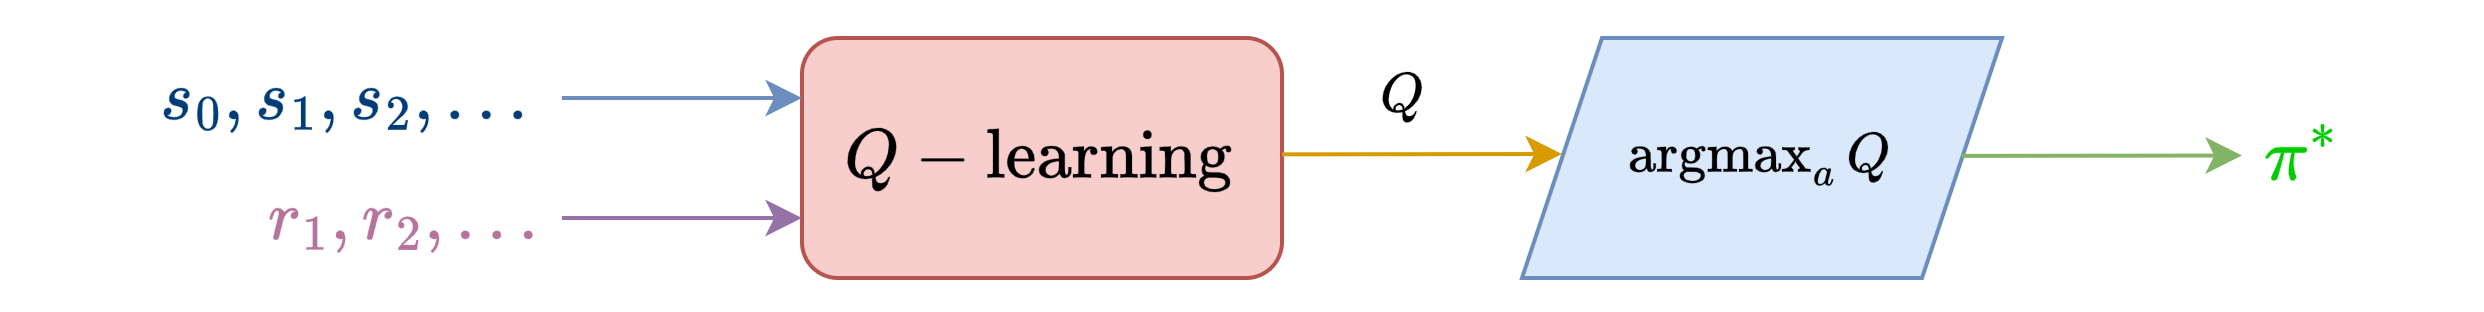
\includegraphics[width=110mm,scale=0.5]{images/rl_images/q_learning.png}
            \caption*{Rather than use $T$ and $R$ to compute $Q$, we compute $Q$ directly.}
        \end{figure}

        Note the major difference:\\

        \begin{clarification}
            \gren{Value iteration} and \purp{$Q$-learning} can seem similar, because they both use our \textbf{model} to compute $Q$.

            The main difference is that:

            \begin{itemize}
                \item Value iteration is used when you \gren{fully understand your model} ($T$ and $R$).

                \item $Q$-learning is used when we have \purp{data points} ($s_t$ and $r_t$).
            \end{itemize}

            In $Q$-learning, we determine $Q$ based on our \orgg{experiences}.
        \end{clarification}

        \phantom{}

        \subsecdiv

        \phantom{}

        How do we do $Q$-learning? Well first, let's remind ourselves of how we traditionally compute $Q$.

        \begin{equation}
            \pur{Q\big(s,a \big)} \;\;=\;\; 
                    R \Big( s,a \Big)
                \;\;+\;\;
                \gamma
                \pur{\sum_{s'}}  
                    \;\;
                    T \Big(          s,a,s' \Big)
                    \;\cdot\; 
                    \bro{ \max_{a'} \Big( \pur{Q\big(s',a' \big)} \Big)}
        \end{equation}

        We don't have $T$ or $R$. But, we can still use the basic idea:

        \begin{itemize}
            \item We take \brow{one action} $a$, and end up going from \redd{state} $s$ to $s'$.
            \item Then, we use the \gren{optimal policy} starting from state $s'$: that's why we take the \pur{$\max$} of $Q$.
        \end{itemize}

        Let's try to apply this to one timestep of our "exploration data":

        \begin{itemize}
            \item We started in state \red{$s_{t-1}$}, and took action \bro{$a_t$}.
            \item We moved to state \red{$s_t$}, and got reward \pur{$r_t$}.
        \end{itemize}

        Our future rewards come from picking the \textbf{best} next action $\org{a_{t+1}}$.

        \begin{figure}[H]
            \centering
            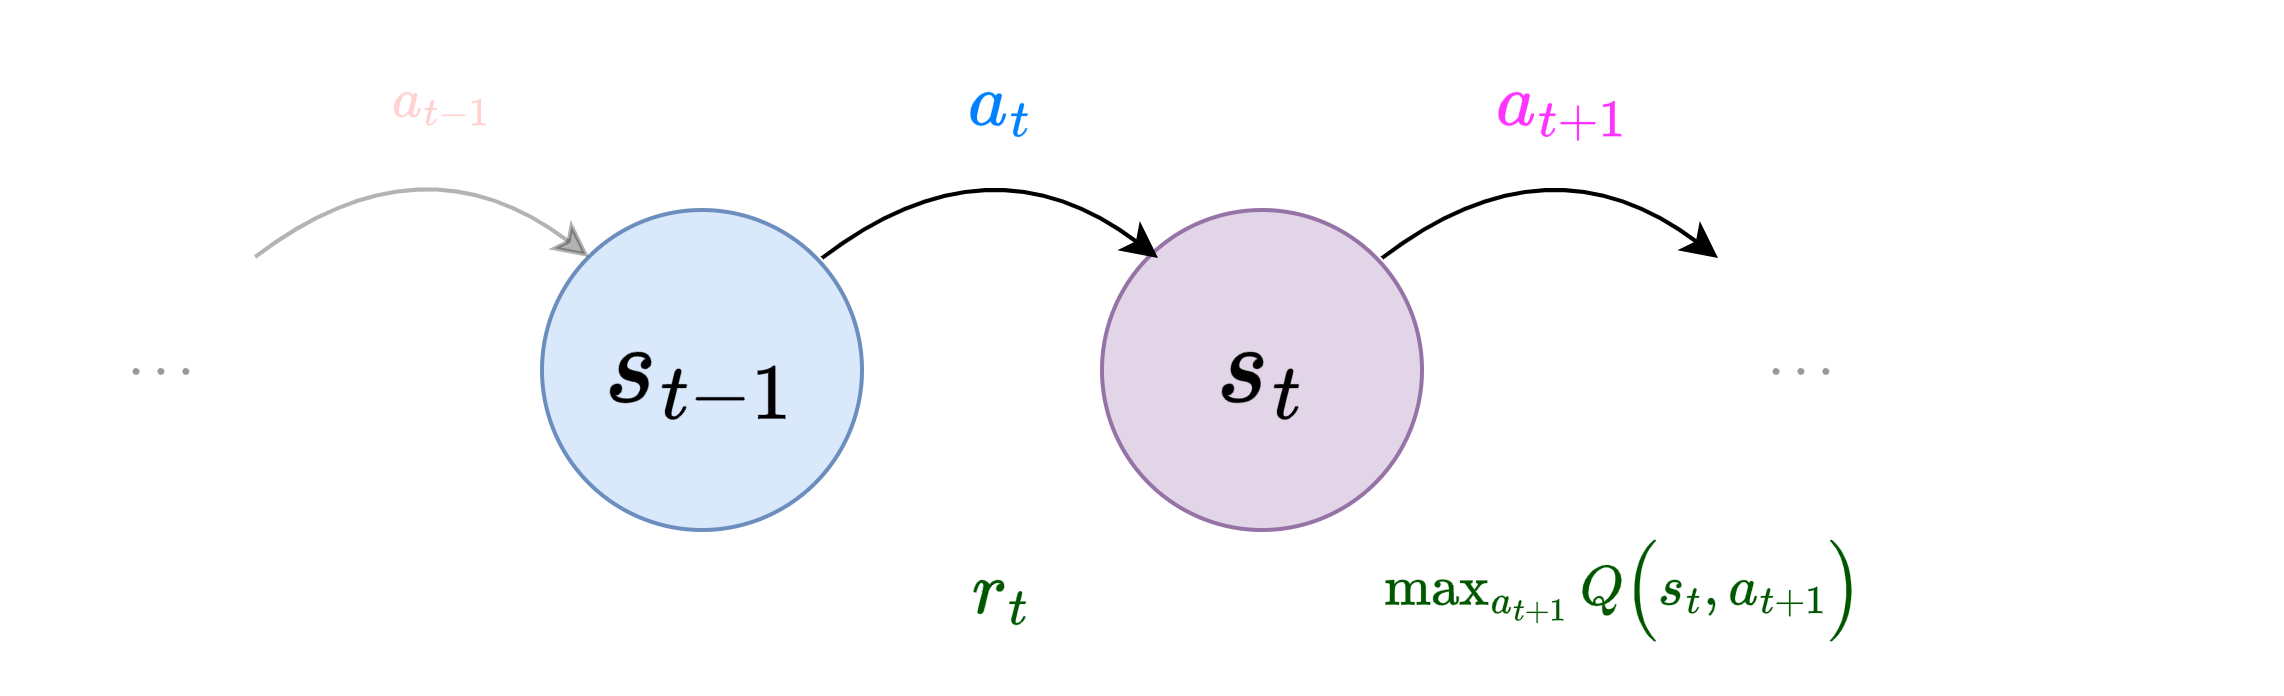
\includegraphics[width=110mm,scale=0.5]{images/rl_images/timestep_data.png}
        \end{figure}

        We'll apply this to our $Q$ equation, to get an \purp{approximation} of $Q$.

        \begin{equation}
            Q_{data}\big(\red{s_{t-1}},\bro{a_t} \big) \;\;=\;\; 
                    \pur{r_t}
                \;\;+\;\;
                \gamma \cdot
                \max_{\org{a_{t+1}}} 
                    \Big( \;\; Q_{old}\big(\blu{s_t},\org{a_{t+1}} \big) \;\; \Big)
        \end{equation}

        Notice that we don't average over possible states ( $\sum_{s'} TQ$):

        \begin{itemize}
            \item This "expected value" was used because we \purp{didn't know} what our next state, $s'$, looked like.

            \item But in this case, we know which state we moved to: \red{$s_t$}.\\
        \end{itemize}

        \begin{kequation}
            When deriving our $Q$-value, we broke our reward into two parts:

            \begin{equation*}
                Q\big(s,a \big) \;\;=\;\;
                \Big(\text{immediate reward}\Big) \;\;+\;\; 
                \Big(\text{future reward}\Big)
            \end{equation*}

            If we apply this to one timestep of our simulation, we get:

            \begin{equation*}
                Q_{data}\big(\red{s_{t-1}},\bro{a_t} \big) \;\;=\;\; 
                        \pur{r_t}
                    \;\;+\;\;
                    \gamma \cdot
                    \max_{\org{a_{t+1}}} 
                        \Big( \;\; Q_{old}\big(\blu{s_t},\org{a_{t+1}} \big) \;\; \Big)
            \end{equation*}
        \end{kequation}


    \phantom{}

    \subsection{$Q$-learning: Making an update rule}

        Now, we have an approximation. But this approximation is only based on one data point. How do we incorporate \orgg{multiple}?

        \begin{itemize}
            \item We could \purp{update} our $Q$-value every time we get new data for that state/action pair.

            \item That way, we can update it repeatedly, to incorporate multiple data points.
        \end{itemize}

        Our current equation doesn't allow us to "update" our $Q$-value, though: it \purp{replaces} it. We'll modify the above equation to get our \vocab{update rule}: 

        

        \begin{itemize}
            \item We want to \gren{average} our new $Q$-value with our old one.
        \end{itemize}
        
        How much do we emphasize our new $Q$-value, versus our old one? We'll represent this with a \textbf{learning rate} $\alpha$.\\

        \begin{definition}
            When we \purp{update} our $Q$-value, our \vocab{learning rate} $\alpha$ ($\alpha \in (0,1]$) tells us how much we emphasize our new $Q$-value, based on \gren{one data point}.

            \begin{itemize}
                \item $(1-\alpha)$ tells us how much we emphasize our old $Q$-value, based on all past data points.
            \end{itemize}

            \begin{equation*}
                Q_{new}\big(\red{s_{t-1}},\bro{a_t} \big) = 
                \alpha \cdot Q_{data}\big(\red{s_{t-1}},\bro{a_t} \big) 
                \;\;+\;\; 
                (1-\alpha) \cdot Q_{old}\big(\red{s_{t-1}},\bro{a_t} \big)
            \end{equation*}
        \end{definition}

        We can also describe $\alpha$ a little more conceptually:\\

        \begin{concept}
            If $\alpha$ is \gren{small} $(\alpha \approx 0)$, we care \gren{very little} about new data.

            If $\alpha$ is \purp{large} $(\alpha \approx 1)$, we are almost entirely \purp{focused on} new data.

            \subsecdiv

            \begin{itemize}
                \item We call this a "\vocab{learning rate}", because it tells us how much we \gren{learn} from new data.
                \item But we could also think of it as a "\vocab{forgetting rate}": in order to learn from new data, we \purp{pay less attention} to older data.
            \end{itemize}
        \end{concept}

        Our equation for $Q$ is going to be messy, so let's change notation:\\

        \begin{notation}
            We update all of our variable names:

            \begin{itemize}
                \item $\red{s=s_{t-1}}$, $\blu{s'=s_t}$, $\bro{a=a_t}$, $\org{a'=a_{t+1}}$, $\pur{r_t=r}$
            \end{itemize}
             
                
            As well as our value function: $\grn{Q=Q_{old}}$
        \end{notation}

        If we plug in our previously calculated $Q_{data}$, we have our $Q$-learning equation:\\

        \begin{kequation}
            In \vocab{$Q$-learning}, all of our $Q$-values start as 0 (similar to value iteration):

            \begin{equation*}
                Q_{new}\big(\red{s},\bro{a} \big) = 0
            \end{equation*}

            With each new data point, we \purp{update} our $Q$ value:

            \begin{equation*}
                Q_{new}\big(\red{s},\bro{a} \big) \quad=\quad  
                (1-\alpha) \cdot Q\big(\red{s},\bro{a} \big)
                \qquad+\qquad 
                \alpha \cdot Q_{data}\big(\red{s},\bro{a} \big)
            \end{equation*}

            \begin{equation*}
                Q_{new}\big(\red{s},\bro{a} \big) \quad=\quad
                    (1-\alpha) \cdot Q\big(\red{s},\bro{a} \big)
                    \qquad+\qquad
                \alpha \cdot 
                \Big( \pur{r}
                    +
                    \gamma \cdot
                    \max_{\org{a'}} 
                        \big( Q\big(\blu{s'},\org{a'} \big) \big) 
                \Big)
            \end{equation*}

            If we're being specific, we sometimes call this approach \vocab{tabular $Q$-learning}.
        \end{kequation}

    \phantom{}

    \subsection{Selecting our action: $\epsilon$-greedy}

        Now, we have a way to \orgg{update} our $Q$-value, based on a data. 

        \begin{itemize}
            \item But we need a way to actually \textbf{get} our data: we need to start \purp{exploring} the space. 
            
            \item Which means our model \gren{decides} what \textbf{data} it wants to \textbf{see}.
        \end{itemize}

        We could try always exploring whichever action seems most optimal. But this is a bad strategy when you're starting out:\\ 

        \begin{concept}
            It's not usually a good idea to \gren{always} use the most "\gren{apparently optimal}" strategy during training.

            \begin{itemize}
                \item There may be plenty of strategies that don't seem good \textit{at first}, but will look more rewarding after some \purp{exploration}.

                \item Your $Q$ values are often very inaccurate, early in training.
            \end{itemize}
        \end{concept}

        \miniex Suppose that there's some treasure at the end of a path.

        \begin{itemize}
            \item You might take 3 steps, and give up: walking around takes work, and you're not immediately rewarded.
            \item You'll miss out on that treasure, because you don't know it's there yet.
        \end{itemize}

        But exploring blindly isn't entirely helpful: it's \textit{too slow}. 
        
        \begin{itemize}
            \item It's often more useful to search near \purp{high-reward} areas: these are more likely to be searched by (and be useful to) a \gren{good policy}. 
            
        \end{itemize}

        This is the \vocab{exploration vs. exploitation problem}.\\

        \begin{definition}
            When we're trying to find the \gren{best policy} for exploring a space, we run into a problem called \vocab{Exploration versus Exploitation}.

            \begin{itemize}
                \item \gren{Exploration}: you're trying to \orgg{learn} more about the space, and you're not as focused on maximizing reward. You \textit{explore} your options.
                
                \item \purp{Exploitation}: based on what you've learned, you want to get the \orgg{maximum reward} from it. You \textit{exploit} your knowledge.
            \end{itemize}

            If you explore more, you might learn how to get better rewards. But if you explore for too long, you'll waste time you could've spent taking advantage of that knowledge.
        \end{definition}

        How much of each should we use? It depends on the context:

        \begin{itemize}
            \item If you only have \redd{10 seconds} left in a game, it might not be worth it to explore anymore: you might as well cash in what you know how to do.

            \item But if you have \gren{5 hours}, you're more likely to find something useful before the game ends: maybe you should explore more.
        \end{itemize}

        For $Q$-learning, our simplest option is to \purp{randomly} alternate between the two modes: \textit{explore} with probability $\epsilon$, and \textit{exploit} with probability $(1-\epsilon)$.\\

        \begin{definition}
            The \vocab{$\eps$-greedy strategy} for $Q$-learning chooses our \gren{actions} for interacting with the environment, \purp{randomly}:

            \begin{itemize}
                \item With probability $\epsilon$, we choose an action $a \in \mathcal{A}$ \gren{uniformly, at random}.
                    \begin{itemize}
                        \item We are equally likely to choose any action: we're \orgg{exploring}.
                    \end{itemize}

                \item With probability $(1-\epsilon)$, we choose the action that gives us the \purp{most reward}, based on what we know:

                    \begin{equation*}
                        \argmax{a \in \mathcal{A}}{ Q(s,a) }
                    \end{equation*}
                    
                    \begin{itemize}
                        \item We're getting the most reward we can: we're \orgg{exploiting}.
                    \end{itemize}
            \end{itemize}
        \end{definition}

        How long do we want to run our $Q$-learning algorithm? It depends on the situation:\\

        \begin{concept}
            We can choose our \vocab{termination condition} for $Q$-learning based on our needs. 

            We could, for example:

            \begin{itemize}
                \item Terminate after a \orgg{fixed} number of timesteps $T$
                \item Terminate when our $Q$-values \purp{aren't changing} much on successive iterations
                \item Terminate if we get \gren{stuck} in the same state, or a loop
            \end{itemize}
        \end{concept}

        \phantom{}

    \subsection{$Q$-learning}

        Based on this, we now have a completed $Q$-learning algorithm:\\

        \begin{definition}
            \vocab{$Q$-learning} is a strategy for learning the $Q$-values of our MDP, so we can find the \gren{optimal policy} for our model.

            We use the following steps:

            \begin{itemize}
                \item We set all $Q$-values to 0. Start from some initial state, $\red{s_0}$.

                \begin{equation*}
                    Q\big(\red{s},\bro{a} \big) = 0
                \end{equation*}

                \item We repeat the following, until we reach our \orgg{termination condition}:

                    \begin{itemize}
                        \item Select an \brow{action} based on $Q$ and current state (possibly with $\epsilon$-greedy)
                            \begin{equation*}
                                \bro{a_t} = \operatorname{select\_action}(Q,\red{s})
                            \end{equation*}

                        \item Record the \purp{result}

                            \begin{equation*}
                                MDP\big(\red{s_{t-1}},\bro{a_t}\big) \;\;=\;\; \org{s_t}\;,\; \pur{r_t}
                            \end{equation*}

                        \item Update our \gren{$Q$-values} accordingly.

                            \begin{equation*}
                                Q\big(\red{s},\bro{a} \big) 
                                \qquad\Longleftarrow\qquad
                                    (1-\alpha) \cdot Q\big(\red{s},\bro{a} \big)
                                    \;\;+\;\;
                                \alpha \cdot 
                                \Big( \pur{r}
                                    +
                                    \gamma \cdot
                                    \max_{\org{a'}} 
                                        \big( Q\big(\blu{s'},\org{a'} \big) \big) 
                                \Big)
                            \end{equation*}
                    \end{itemize}
                \item Compute our \gren{policy} based on $Q$.
            \end{itemize}
            
        \end{definition}

            \note{$select\_action$ isn't a specific function: in our case, it could just be $\epsilon$-greedy. But we could choose other options.}


        $Q$-learning is guaranteed to \purp{converge} under surprisingly simple conditions:\\

        \begin{theorem}
            $Q$-learning \vocab{converges} if 

            \begin{itemize}
                \item Over an \purp{infinitely-long run}, we visit every state an \gren{infinite number of times}.
            \end{itemize}

            With this requirement, we ensure that our model doesn't decide on a sub-optimal strategy, without checking out other possibilities.
        \end{theorem}

            \note{Okay, so an infinite amount of time isn't exactly promised to us... but it's better than a lot of other stricter convergence requirements!}

        Guaranteed convergence does require our learning rate $\alpha$ to \orgg{decay}, or gradually shrink over time.

        \begin{itemize}
            \item But typically, we set $\alpha$ to a constant, for convenience.
                \note{We can set it to decay, but this also slows down the learning process.}
        \end{itemize}

    \pagebreak

        Now that we have our completed $Q$-learning strategy, let's go through some details that we skipped over.

    \subsection{Initialization}

        When we're starting our $Q$-learning process, we have to choose some initial state, $s_0$.

        \begin{itemize}
            \item For some problems (like a chess game), there's a \gren{natural choice} of initial state.
            \item For other problems (like a robot moving across terrain), there may be \purp{multiple} possible "initial states". 
        \end{itemize}

        In the latter case, we often \purp{randomly} select our initialization.\\

        \begin{concept}
            When we're uncertain what \redd{initial state $s_0$} to use, we often \purp{randomly sample} from our state space.
        \end{concept}

        This choice of initialization often \gren{biases} what we learn about the state space: which sections we \textbf{visit}, what we \textbf{learn}, etc.

        So, it's often helpful to run $Q$-learning through \purp{several initializations}: we have one "run" of our MDP for each initialization.

        \begin{itemize}
            \item So we don't lose all of our progress, we usually modify it so that our $Q$-table (computed $Q$ values) is \textbf{carried over} between different "runs".\\
        \end{itemize}

        \begin{concept}
            To explore our \gren{state-action space} (possible options) more thoroughly, we may take \purp{several different paths} through our MDP.

            \begin{itemize}
                \item Each path starting with a \redd{different initialization}, $s_0$.
            \end{itemize}

            We \orgg{share} our $Q$-values between these "runs" of our MDP, so that we can build up a more complete representation of the environment.
        \end{concept}


    \phantom{}

    \subsection{Action and state space}

        Our previous approach to $Q$-learning assumes that our \brow{action space} and \redd{state space} are both \textbf{discrete}.

        \begin{itemize}
            \item But this might not always be a realistic assumption. We might need a \vocab{continuous} space.\\
        \end{itemize}

        \begin{concept}
            Our above approach to $Q$-learning is called \vocab{tabular $Q$-learning}. 

            It assumes that we have a \purp{discrete} (typically finite) \redd{state space} and \brow{action space}.

            \begin{itemize}
                \item Other versions of $Q$-learning, on the other hand, allow this space it be \vocab{continuous}.
            \end{itemize}
        \end{concept}

            \note{We call it "tabular $Q$-learning" because our values could be stored in a \gren{table}.}

        \miniex A discrete state space might be $\setty{1,2,3,4,5,6}$. A continuous one might be $\big[1,6\big]$.

        \begin{itemize}
            \item $1+\sqrt{2}$ is allowed in the latter, but not the former.
        \end{itemize}

        This causes us problems, though: if we have a continuous state/action space, we have an \gren{infinite} number of possible states/actions.

        \begin{itemize}
            \item It's impossible to get the $Q$-values for all of these state-action pairs.
        \end{itemize}

        Many $Q$-learning variations enable continuous action/state spaces. Later, we'll focus on one example: \vocab{Deep $Q$-learning}.




    \phantom{}

    \subsection{An alternate view of $Q$-learning (\redd{Optional})}

        Consider our basic, conceptual $Q$-learning equation:
            \note{We're averaging our immediate data, with our past experience with this $Q$-value.}

        \begin{equation}
            Q_{new}\big(\red{s},\bro{a} \big) \quad=\quad  
            (1-\alpha) \cdot Q\big(\red{s},\bro{a} \big)
            \qquad+\qquad 
            \alpha \cdot Q_{data}\big(\red{s},\bro{a} \big)
        \end{equation}

        We get something interesting if we rearrange it:

        \begin{equation}
            Q_{new}\big(\red{s},\bro{a} \big) \quad=\quad  
            Q\big(\red{s},\bro{a} \big)
            \;\;+\;\; 
            \alpha
            \Big( 
                Q_{data}\big(\red{s},\bro{a} \big) - Q\big(\red{s},\bro{a} \big)   
            \Big)
        \end{equation}

        The right term could be seen as the \purp{disagreement} between our new data, and past experience.
        

        \begin{itemize}
            \item And thus, $\alpha$ tells us how much we \purp{care} about that disagreement, and want to account for it.
        \end{itemize}

        \begin{equation}
            Q_{new}\big(\red{s},\bro{a} \big) \quad=\quad  
            Q\big(\red{s},\bro{a} \big)
            \;\;+\;\; 
            \alpha
            \overbrace{
            \Big( 
                Q_{data}\big(\red{s},\bro{a} \big) - Q\big(\red{s},\bro{a} \big)   
            \Big)
            }^{\text{"Error" of our old answer}}
        \end{equation}

        This is an \purp{update rule}: the difference between our new and old answer decides how we want to update.

        \begin{concept}
            We can view \vocab{$Q$-learning} as a direct \orgg{update rule}:
            
            \begin{itemize}
                \item We "update" our current $Q$ value based on the \purp{difference} from what the \gren{newest data point} predicts.
            \end{itemize}

            \begin{equation*}
                Q_{new}\big(\red{s},\bro{a} \big) \quad=\quad  
                Q\big(\red{s},\bro{a} \big)
                \;\;+\;\; 
                \alpha
                \overbrace{
                \Big( 
                    Q_{data}\big(\red{s},\bro{a} \big) - Q\big(\red{s},\bro{a} \big)   
                \Big)
                }^{\text{"Error" of our old answer}}
            \end{equation*}
        \end{concept}

        


        

        



    \pagebreak

    \subsection{Problems with $Q$-learning: Slow Convergence}

        Because $Q$-learning only updates one state-action pair at a time, it often \gren{converges slowly}.

        Let's see an example: 

        \begin{itemize}
            \item \miniex We'll re-use our example of going down a long hallway, with treasure at the end.
            \item Each "state" is one tile of the hallway. We'll arrange them \gren{left-to-right}: we can move left or right down the hallway. We start on $s_0$.
        \end{itemize}

        \begin{figure}[H]
            \centering
            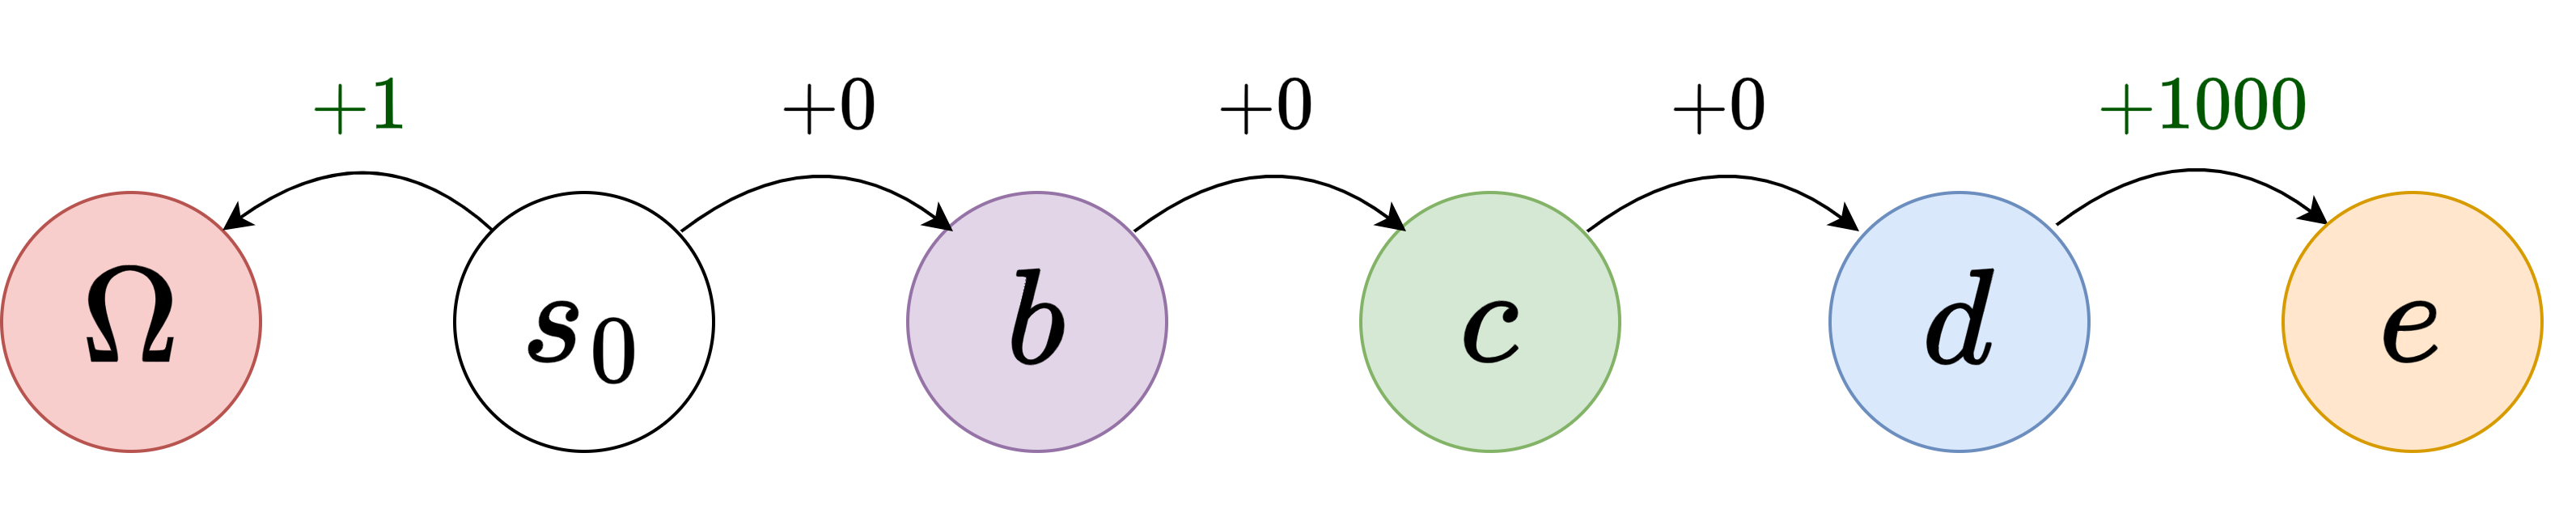
\includegraphics[width=100mm,scale=0.5]{images/rl_images/hallway.png}
            \caption*{Above the arrows, we can see the reward we get for going left/right in each state.}
        \end{figure}
        
        If we go left, we get a small reward. If we go right, we'll \textit{eventually} get a huge reward.
            \note{Assume that every state transition we don't show (left/right) is +0.}

        Being able to see from above, it's obvious to us that going \orgg{right} is better. But what does the robot see?
            \note{So long as $\gamma$ isn't really small: if our model is really likely to fail after 1 or 2 steps, then the right reward isn't worth it.}

        \begin{itemize}
            \item Go right once. \redd{No reward.}
            \item Go left once. \gren{Reward!}
            \item We should go left!\\
        \end{itemize}

        \begin{concept}
            At first, our $Q$-learning algorithm will prioritize \purp{short-term} rewards over long-term rewards.

            \begin{itemize}
                \item It hasn't had time to \gren{find} rewards further from $s_0$.
            \end{itemize}
        \end{concept}

        Well, as the robot explores, it'll learn to get the reward, right? Let's see what happens as we move right, to our $Q$ values.

        \begin{equation}
            Q\big(s,a \big) 
            \qquad\Longleftarrow\qquad
                (1-\alpha) \cdot Q\big(s,a \big)
                \;\;+\;\;
            \alpha \cdot 
            \Big( r
                +
                0.9 \cdot
                \max_{a'} 
                    \big( Q\big(s',a' \big) \big) 
            \Big)
        \end{equation}

        For simplicity, we'll use $\alpha=1$, $\gamma=0.9$.

        \begin{equation}
            Q\big(\red{s},\bro{a} \big) 
            \qquad\Longleftarrow\qquad 
                \pur{r}
                +
                0.9 \cdot
                \max_{\org{a'}} 
                    \big( Q\big(\blu{s'},\org{a'} \big) \big) 
        \end{equation}

        Based on this model, our reward for going left ($\leftarrow$) is simple:

        \begin{equation}
            Q\big(s_0,\; \leftarrow\big)=\grn{+1}
        \end{equation}

        Let's go \orgg{right} ($\rightarrow$) instead.

        \begin{itemize}
            \item Move from $s_0$ to \pur{$b$}: no reward. $Q\big(s_0,\; \rightarrow\big)=0$
            \item Move from \pur{$b$} to \grn{$c$}: no reward. $Q\big(b,\; \rightarrow\big)=0$
            \item Move from \grn{$c$} to \blu{$d$}: no reward. $Q\big(c,\; \rightarrow\big)=0$
            \item Move from \blu{$d$} to \org{$e$}: reward! $Q\big(d,\; \rightarrow\big)=\grn{+1000}$
        \end{itemize}

        \begin{figure}[H]
            \centering
            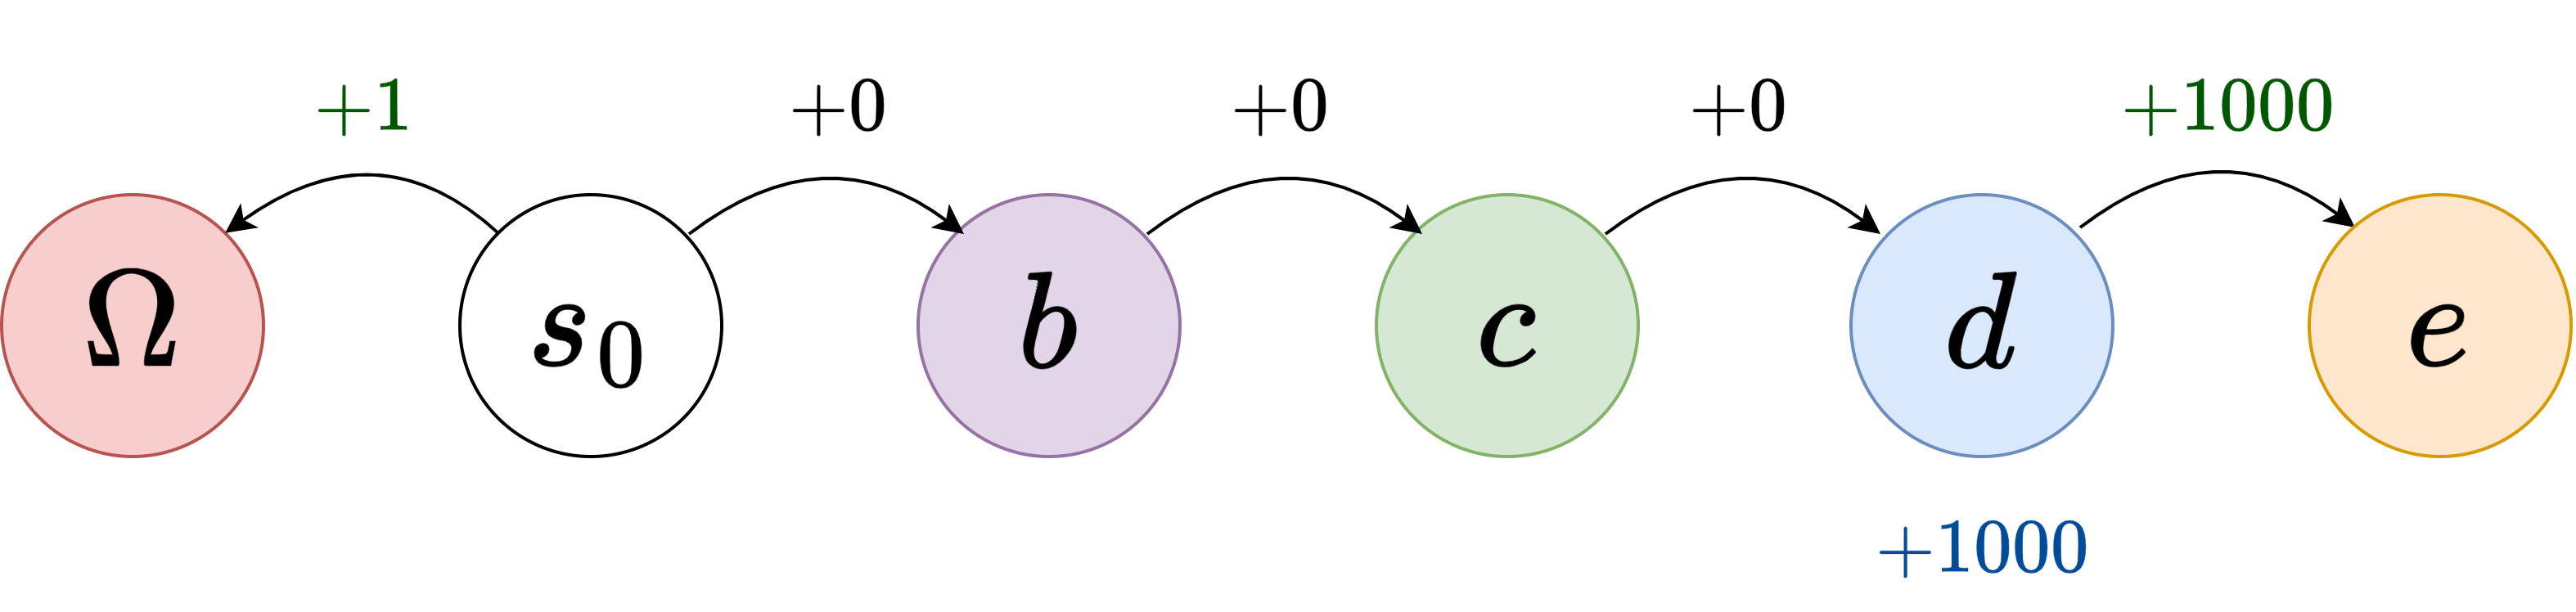
\includegraphics[width=100mm,scale=0.5]{images/rl_images/hallway_d.png}
            \caption*{We learned that $d$ is able to produce a +1000 reward.}
        \end{figure}

        We did it! We learned something, at the very end. Will our robot go the way we want?

        \begin{itemize}
            \item We start over from $s_0$. Let's \purp{compare} the left and right rewards.

            \begin{equation}
                Q\big(s_0,\; \leftarrow\big)=\grn{+1} \qquad \qquad Q\big(s_0,\; \rightarrow\big)=0
            \end{equation}

            \item Let's go left again!
        \end{itemize}

        No luck -- it still prefers the \gren{short-term} reward.\\

        \begin{concept}
            Even once we find a reward, $Q$-learning will only update that \gren{single state-action pair}.

            \begin{itemize}
                \item That means that nearby states, \purp{don't know} about that reward!
            \end{itemize}

            We have to run $Q$-learning through a nearby state \textit{again} to find the reward.
        \end{concept}

        So, let's take another journey:

        \begin{itemize}
            \item Move from $s_0$ to \pur{$b$}: no reward. $Q\big(s_0,\; \rightarrow\big)=0$
            \item Move from \pur{$b$} to \grn{$c$}: no reward. $Q\big(b,\; \rightarrow\big)=0$
            \item Move from \grn{$c$} to \blu{$d$}: no reward. \redd{However}, $Q$ \purp{remembers} that $d$ can provide a reward!

            
        \end{itemize}

        \begin{equation*}
            Q\big(\red{c}, \; \bro{\rightarrow} \big) 
            \qquad\Longleftarrow\qquad 
            \pur{r}
            +
            0.9 \cdot
            \max_{\org{a'}} 
                \big( Q\big(\blu{d},\org{a'} \big) \big) 
        \end{equation*}

        \begin{equation*}
            Q\big(\red{c}, \; \bro{\rightarrow} \big) 
            \qquad\Longleftarrow\qquad 
            \pur{0}
            +
            0.9 \cdot
            \overbrace{
                 Q\big(\blu{d},\org{\rightarrow} \big) 
            }^{\grn{+1000}}
            = \grn{+900}
        \end{equation*}

        We know that $d$ is valuable. Thus, we've learned that $c$ is valuable, because it's attached to $d$. 

        \begin{figure}[H]
            \centering
            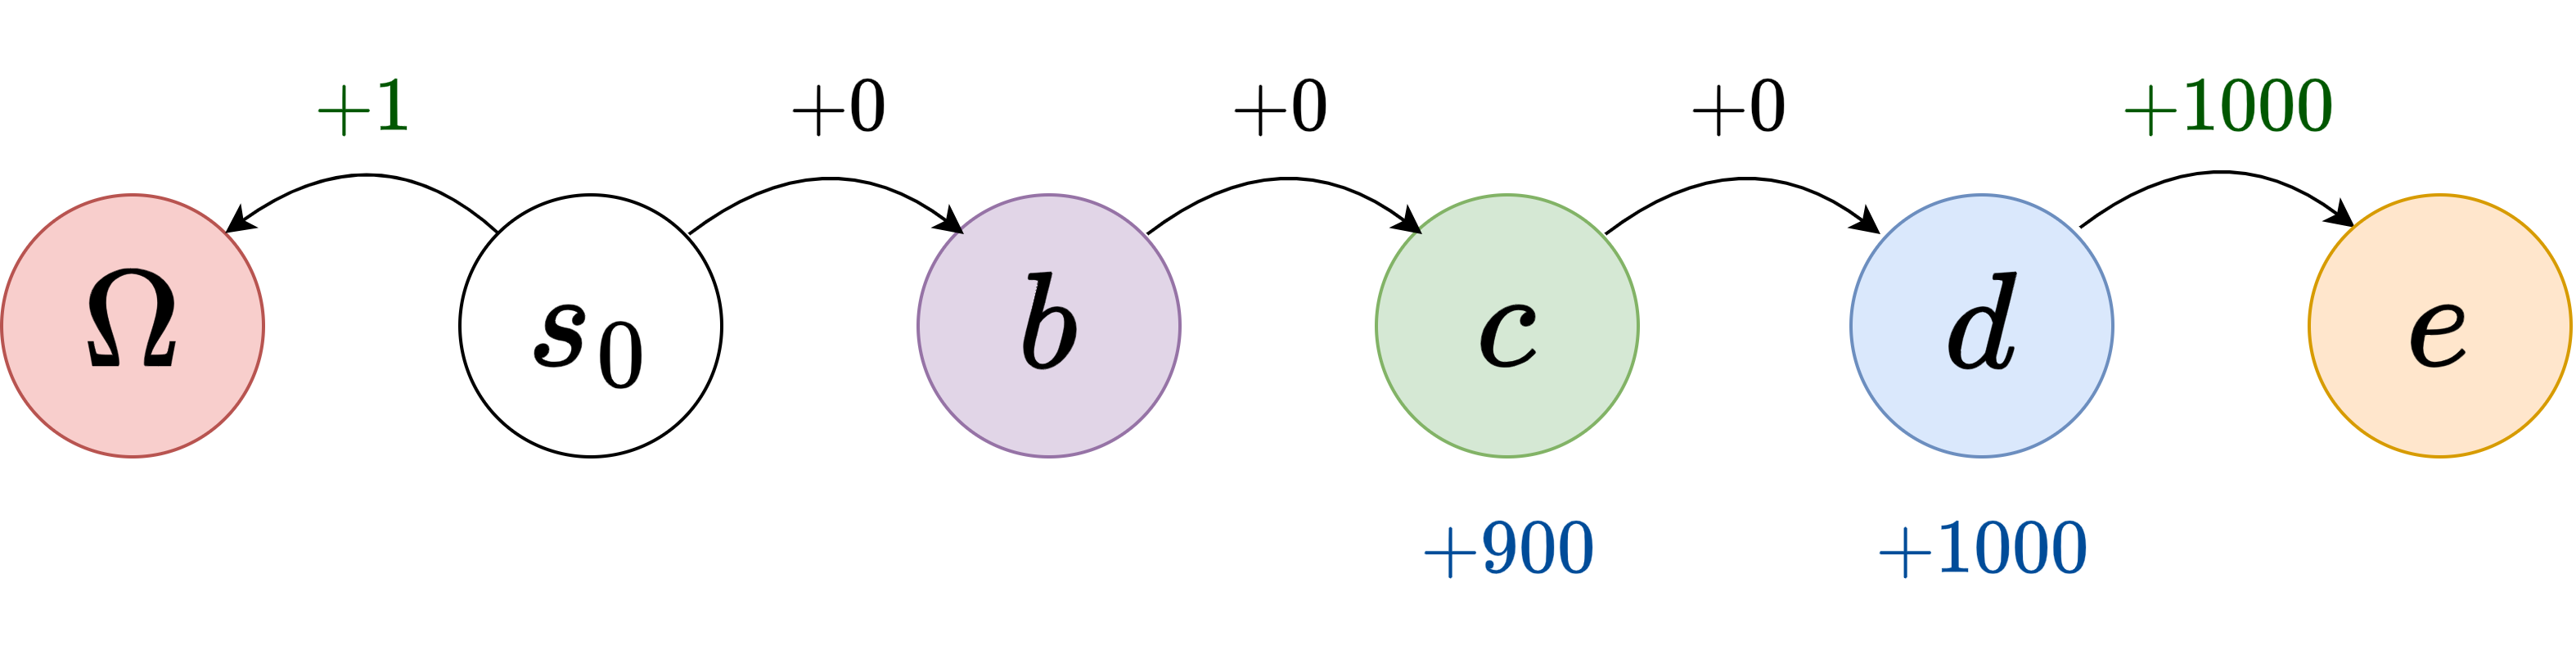
\includegraphics[width=100mm,scale=0.5]{images/rl_images/hallway_c.png}
            \caption*{It's worth visiting $c$, because it allows you to visit $d$.}
        \end{figure}

        \begin{concept}
            Each time that we run though a path to a reward, \purp{one more state} learns about the reward.

            \begin{itemize}
                \item If state $d$ has an \brow{action} with a \purp{reward}, then \gren{$d$ is \gren valuable}.
                \item If state $c$ can move to $d$, \gren{$c$ is valuable}, because it gives a \purp{path to reach $d$}.
                \item If state $b$ can move to $c$, \gren{$b$ is valuable}, because it gives a \purp{path to reach $c$}.
                \item This repeats until we reach $s_0$.
            \end{itemize}

            Each $Q$-learning run will update one more state.
        \end{concept}

        If we continue, we get the result we're looking for:

        \begin{figure}[H]
            \centering
            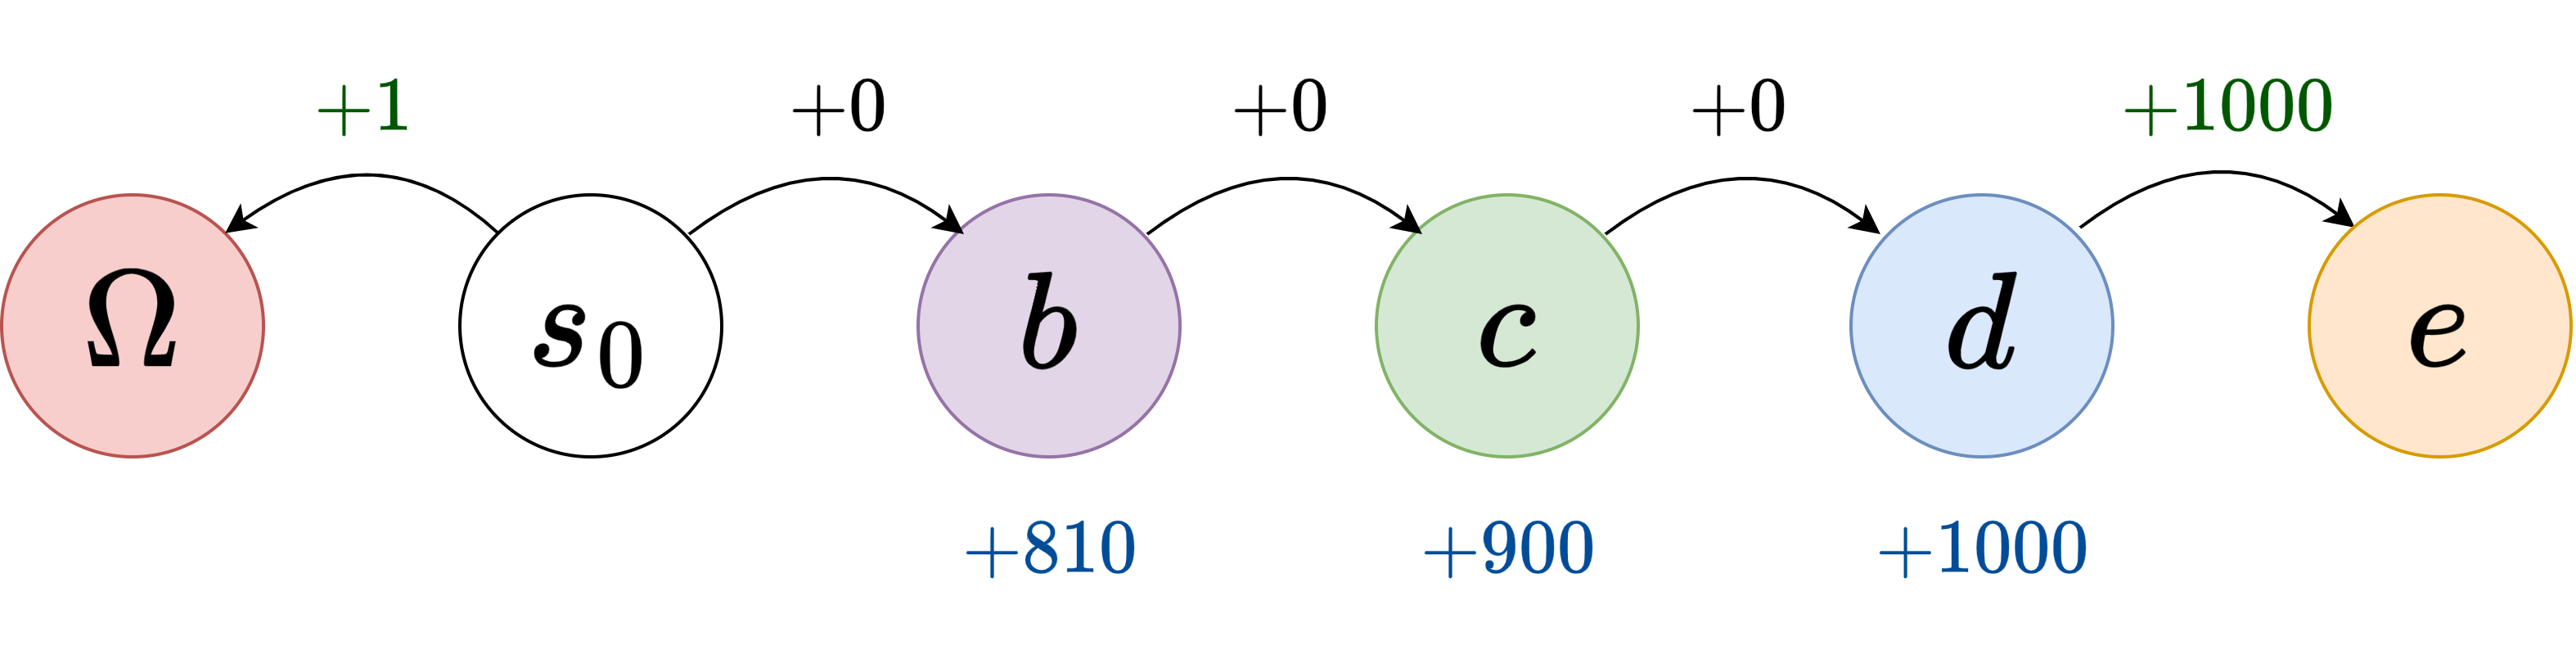
\includegraphics[width=100mm,scale=0.5]{images/rl_images/hallway_b.png}
            \caption*{We can now see that $b$ has a lot of value. (The bottom number is the "expected value" we can get after reaching state $s$, if we make the best choice.)}
        \end{figure}

        Let's compute $Q(s_0,\rightarrow)$, now that we know $b$ is valuable:

        \begin{equation}
            Q\big(s_0,\; \leftarrow\big)=\grn{+1} \qquad \qquad Q\big(s_0,\; \rightarrow\big)=\grn{+729}
        \end{equation}

        Finally, we go right!

        \begin{itemize}
            \item But it took 4 trips right before we knew that.
        \end{itemize}

        This is already annoying, but it can get even worse: suppose we only reached the reward after moving right \redd{10 times}.

        \begin{figure}[H]
            \centering
            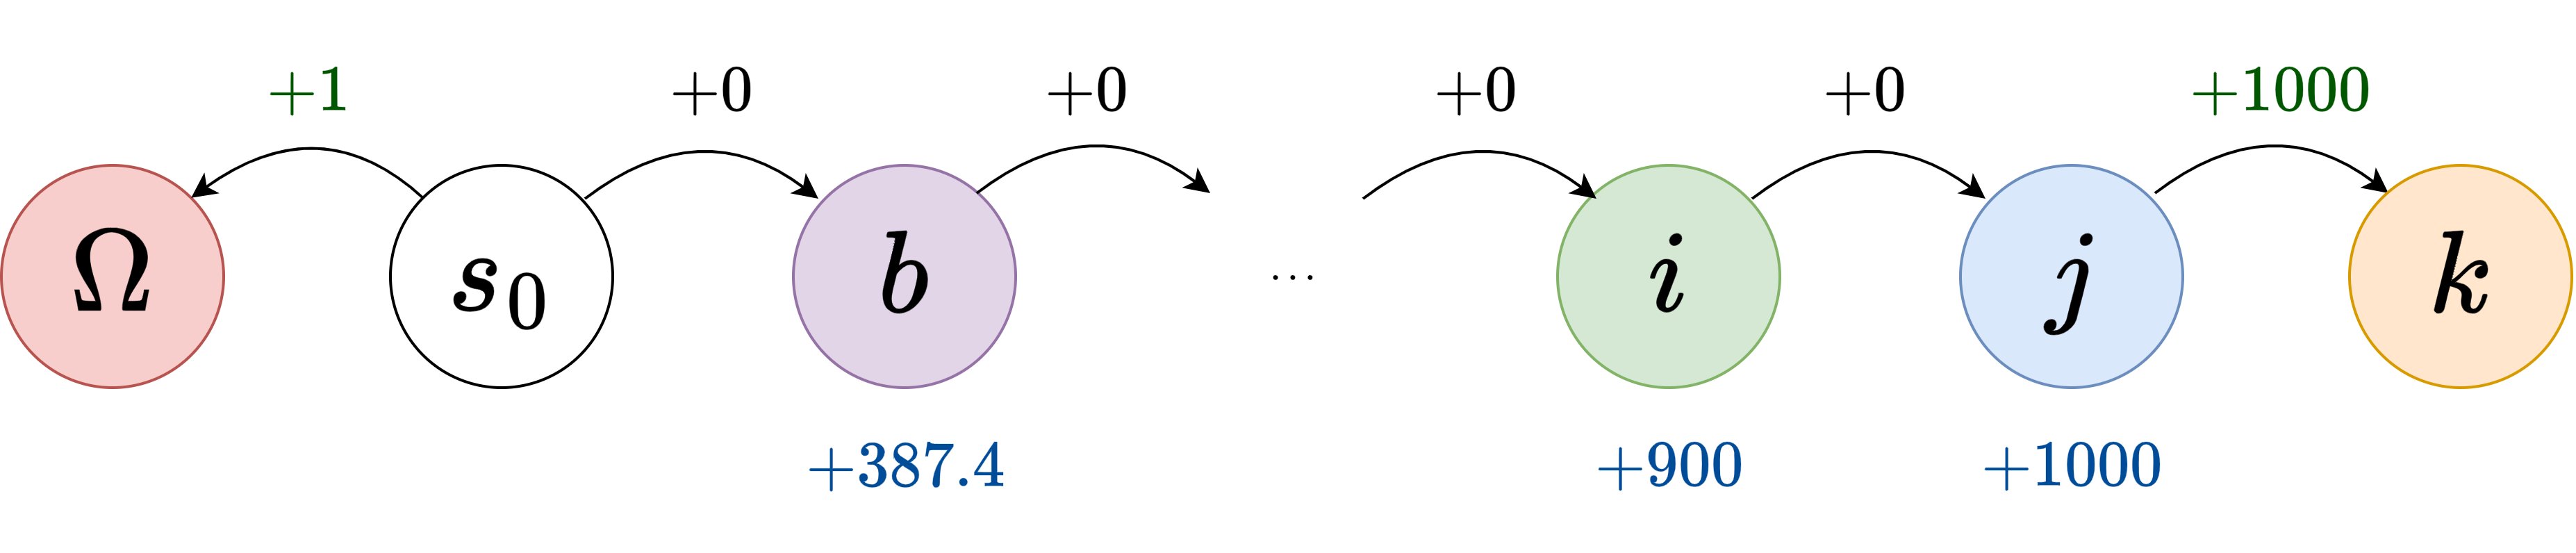
\includegraphics[width=100mm,scale=0.5]{images/rl_images/long_hallway.png}
            \caption*{It's still worth it to go right, but it takes a painfully long time to figure that out.}
        \end{figure}

        Instead of making 4 trips right, we'll have to make 10 trips right.
            \note{Each trip is, thankfully, shorter than the last. But that's still really slow.}

        \begin{itemize}
            \item And imagine if the "reward" for going right was \red{-1} instead of +0.
            \item Our model would \textit{always} prefer to go left, until the very end. Which means, it only has an $\epsilon/2$ chance of moving right.
                \note{$\epsilon$ chance to move in a random direction, and 1/2 chance to randomly move right.}

            \item Going right $n$ times in a row has a chance of $(\epsilon/2)^n$. 
        \end{itemize}

        \begin{figure}[H]
            \centering
            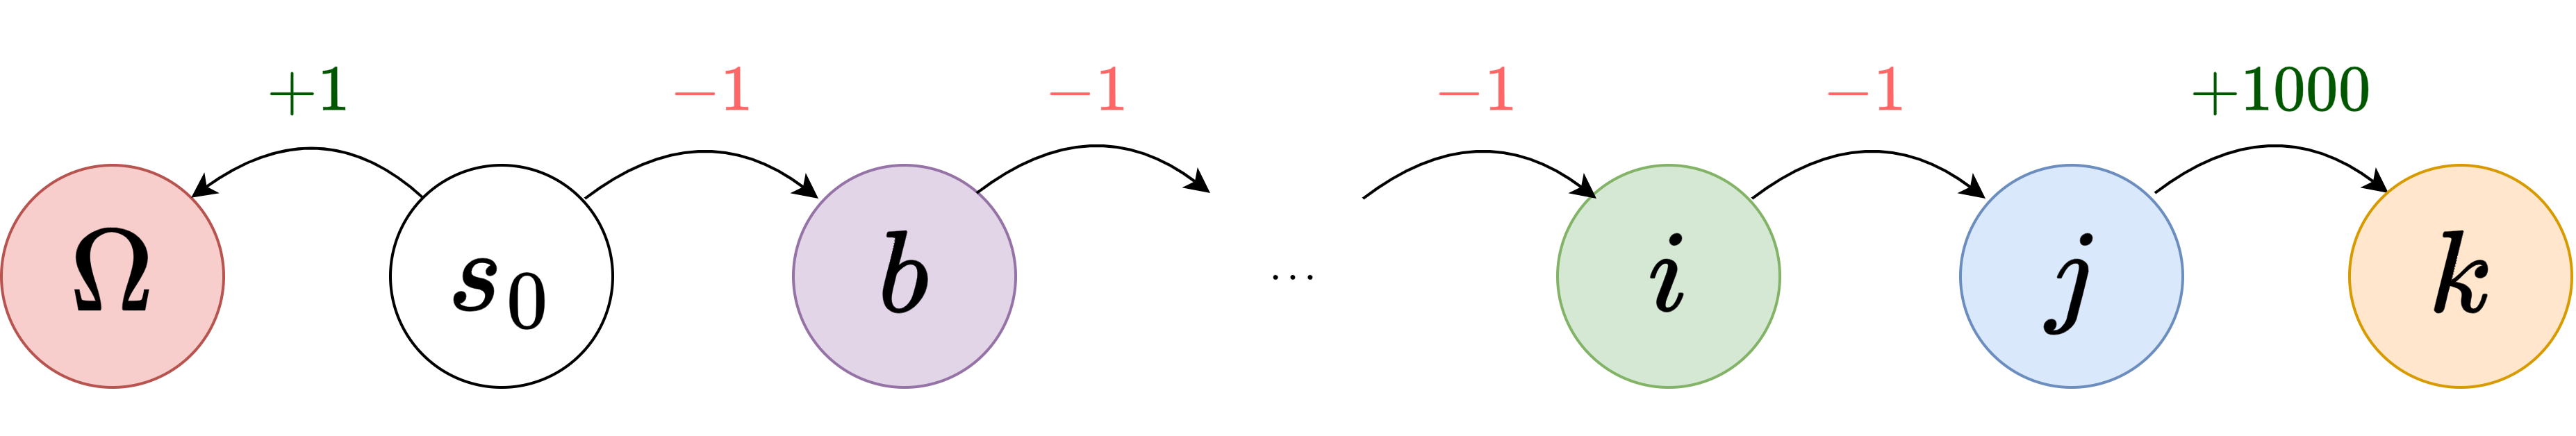
\includegraphics[width=100mm,scale=0.5]{images/rl_images/painful_hallway.png}
            \caption*{If moving left from $(b,c,d...)$ is still $+0$, our model will try to avoid going right. It's even harder to make progress, now.}
        \end{figure}

        \begin{concept}
            The \gren{longer} it takes to reach a distant reward, the more \purp{difficult} it is to \orgg{propagate} that information back to $s_0$.

            \begin{itemize}
                \item This shows how \textit{inefficient} $Q$-learning can be: only updating one \gren{state-action} pair at a time, means that information travels \purp{slowly} between states.
            \end{itemize}
        \end{concept}

        

        

        
        


    



    \pagebreak

    \subsection{Deep $Q$-learning}

        Earlier, we mentioned that our state space $\mathcal{S}$ and action space $\mathcal{A}$ are \purp{discrete} and relatively \purp{small}.

        \begin{itemize}
            \item But what do we do if we need them to be \gren{continuous}?
                \note{Or, just very large? A large finite space is still a pain.}

        \end{itemize}

        One solution is to treat $Q$ like any other continuous variable we want to \purp{predict}.

        \begin{itemize}
            \item What do we do with complicated, continuous variables we want to predict? We use \vocab{neural networks}.\\
        \end{itemize}

        \begin{definition}
            In \vocab{Deep $Q$-Learning}, we use \purp{deep neural networks} to predict $Q$-values: a \orgg{regression} problem.

            \begin{itemize}
                \item This approach allows us to handle \gren{continuous} state and action spaces.
            \end{itemize}

            \subsecdiv

            To teach this network, we train it the way that we train any neural network, using data we receive while exploring:
            
            \begin{itemize}
                \item Input: \redd{states} and/or \brow{actions}
                \item Output: expected \purp{reward}, $Q_{NN}$.
            \end{itemize}
            
        \end{definition}

        Our goal is to make the most accurate predictions of the $Q$-value. We determine $Q$ based on each data point, 

        \begin{equation}
            Q_{data}\big(\red{s_{t-1}},\bro{a_t} \big) \;\;=\;\; 
                    \pur{r_t}
                \;\;+\;\;
                \gamma \cdot
                \max_{\org{a_{t+1}}} 
                    \Big( \;\; Q\big(\blu{s_t},\org{a_{t+1}} \big) \;\; \Big)
        \end{equation}

        So, we want our predicted $Q$ value ($Q_{NN}$) to be \purp{as close} to $Q_{data}$ as possible.\\

        \begin{definition}
            Our \vocab{deep $Q$-learning} neural network will use \purp{squared error}:

            \begin{equation*}
                \Big( Q_{NN}(\red{s},\bro{a}) - Q_{data}(\red{s},\bro{a}) \Big)^2
            \end{equation*}
            

            In other words, our goal is for our NN ($Q_{NN}$) to match the $Q$-values of our data points ($Q_{data}$), as close as possible.

            \begin{equation*} 
                \Bigg( Q_{NN}(\red{s},\bro{a}) - \Big(\pur{r}
                    \;\;+\;\;
                    \gamma \cdot
                    \max_{\org{a_{t+1}}} 
                     Q_{NN}\big(\blu{s'},\org{a'}  \big)\Big) \;\; \Bigg)^2
            \end{equation*}
        \end{definition}

        \subsecdiv

        Note that, in our definition, we said states \orgg{and/or} actions: we might not have both as the input to our neural network. How?\\

        \begin{concept}
            There are three main ways we can design our \vocab{neural network}: in all cases, $Q(\red{s},\bro{a})$ is the \gren{output}.

            \begin{itemize}
                \item Each \brow{action $a$} has a separate neural network. \redd{State $s$} is the input.
                    \begin{itemize}
                        \item This only works with a \brow{small, discrete action space}.
                    \end{itemize}

                    \item Each \redd{state $s$} has a separate neural network. \brow{Action $a$} is the input.
                    \begin{itemize}
                        \item This only works with a \redd{small, discrete state space}.
                    \end{itemize}

                    \item We have one neural network shared by \textbf{all inputs}. \redd{State $s$} and \brow{action $a$} are \textit{concatenated} into the input. 
                    \begin{itemize}
                        \item This one is the most flexible, but it's \purp{very hard} to find $\argmax{\bro{a}} Q(\red{s},\bro{a})$.
                    \end{itemize}
            \end{itemize}
        \end{concept}

        \begin{figure}[H]
            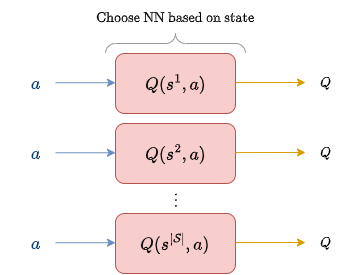
\includegraphics[width=70mm,scale=0.5]{images/rl_images/state_nns.png}
            \quad
            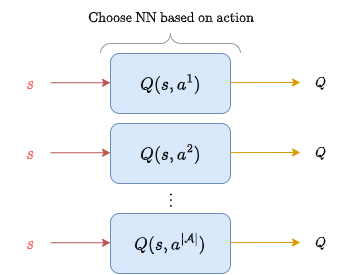
\includegraphics[width=70mm,scale=0.5]{images/rl_images/action_nns.png}
            \caption*{In one system, each \redd{state $s^i$} has its own neural net. In the other system, each \brow{action $a^j$} has its own neural net.}
        \end{figure}

        \begin{figure}[H]
            \centering
            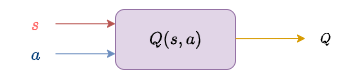
\includegraphics[width=70mm,scale=0.5]{images/rl_images/single_nn.png}
            \caption*{This version works for continuous state/action spaces, but comes with its own difficulties.}
        \end{figure}

        Unfortunately, deep $Q$-learning is often pretty unstable.
            \note{Improving, and then getting worse, for example.}

        \begin{itemize}
            \item But it's still useful enough to try, in a lot of contexts.
        \end{itemize}




    \phantom{}

    \subsection{Catastrophic Forgetting}

        Here, we'll address one of these forms of \textbf{instability}.

        \begin{itemize}
            \item When training a typical neural network, all of our data is \vocab{IID}: independent, and coming from the same distribution.
            \item But this is \purp{not} the case for $Q$-learning.\\
        \end{itemize}

        \begin{concept}
            In $Q$-learning, our data are \orgg{correlated in time} ("temporally correlated"). Meaning, \gren{timing} affects our data.

            \begin{itemize}
                \item Why? Because two \redd{states} which are "\purp{near}" each other, typically behave \gren{similarly}.
                \item If the \orgg{time} between two data points is \purp{short}, they're probably \gren{nearby} in state space. So, they're more likely to be similar.
            \end{itemize}
        \end{concept}

        \miniex Consider a robot moving across the earth.

        \begin{itemize}
            \item \gren{Example 1:} If, at time $t$, our robot is on a \textbf{mountain}, it's more likely to be on a mountain at $(t-1)$ and $(t+1)$.
            \item \gren{Example 2:} The 12 hours of daytime may seem very different from the 12 hours of nighttime.
        \end{itemize}

        Why is this a problem? Because our neural network adjusts $Q$ based on \purp{new data}.

        That means that our NN is capable of \gren{forgetting}: if there's been a long time since we've used some information, it will be replaced by information from a \orgg{different context}.\\

        \begin{definition}
            \vocab{Catastrophic forgetting} occurs when our neural network hasn't seen a certain type of data in a long time, and \orgg{forgets} how to do a task.

            \begin{itemize}
                \item In deep $Q$-learning, it can occur when \purp{recent} data doesn't reflect \gren{past} data.

                \item So, our model \textit{forgets} about the portion of the state space it visited in the past.
            \end{itemize}
        \end{definition}

        \begin{figure}[H]
            \centering
            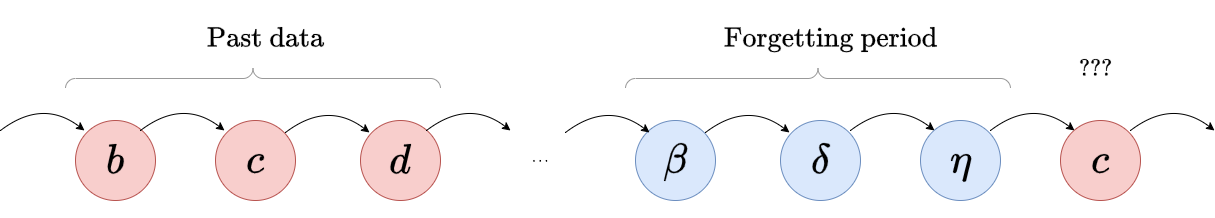
\includegraphics[width=130mm,scale=0.5]{images/rl_images/catastrophic forgetting.png}
            \caption*{When we return to the red region, we've forgotten what we learned the first time!}
        \end{figure}

        This is still a problem, even if we don't return to the red region during this MDP run:

        \begin{itemize}
            \item It could be important for future runs.
        \end{itemize}




    \phantom{}

    \subsection{Experience Replay}

        What do we do if a person is worried about forgetting something? You \purp{remind} them of the past information.

        \begin{itemize}
            \item Perhaps they talk about that memory, or you periodically mention it to them.
        \end{itemize}

        This is our solution: we \gren{keep track} of these past experiences, and re-use them later: we essentially "refresh" our NN, so that it doesn't forget.

        This is called \vocab{experience replay}.\\

        \begin{definition}
            \vocab{Experience replay} is a technique for addressing \purp{catastrophic forgetting}.

            \begin{itemize}
                \item In experience replay, we store our \gren{past experiences} $(s,a,s',r)$ in a \vocab{replay buffer}.

                \item This buffer is used to "\purp{remind}" our NN of past events.
            \end{itemize}

            After every timestep, we do two things:

            \begin{itemize}
                \item We store our newest experience in our replay buffer.

                \item We \gren{randomly} pull $n$ memories from our replay buffer, and "\purp{re-experience}" them: we re-train our model, based on these past events.
            \end{itemize}
        \end{definition}

        This storage can get painfully large, though. This can be problematic:

        \begin{itemize}
            \item If the memories are too far back, they may just \purp{not be relevant} anymore: they're in an undesirable part of the state space.
            \item It becomes \gren{expensive} to store all of those memories.
        \end{itemize}

        So, we tend to only keep some of them.\\

        \begin{definition}
            Rather than storing \textit{every} event in our \purp{replay buffer}, we only keep the \gren{$k$ most recent memories}, in a \vocab{sliding window}.

            \begin{itemize}
                \item This prevents our memory from getting \gren{too full}, or focusing on memories that are \orgg{too old}.
            \end{itemize}

           

            The best \gren{size} for our sliding buffer \purp{depends} on the problem, and what our state space is like.
        \end{definition}


        Another reason that we like \vocab{experience replay} is for improving on a weakness we mentioned before:\\

        \begin{concept}
            Randomly reviewing \gren{old memories} has a second benefit: it allows us to \purp{propagate rewards} between states faster.

            \begin{itemize}
                \item Previously, we only updated \orgg{one state-action value}, for each experience.
                \item This means that, when we get our \purp{reward}, we \redd{only} update the state $s_r$ we got the reward in.
            \end{itemize}

            With experience replay, we're more likely to \orgg{revisit} a state $s_n$ "near" our reward:
            
            \begin{itemize}
                \item If $s_n$ is near $s_r$, then $s_n$ is more valuable, for being a \purp{path} to the reward.
            \end{itemize}

        \end{concept}

            \note{By "nearby", we mean that there's an short series of actions $a_t$ that moves us from $s_n$ to $s_r$.}

        \miniex This might, for example, help speed up the hallway problem.
            \note{The one we used earlier in the chapter.}

       



    \pagebreak 

    \subsection{Fitted $Q$-learning}

        Here, we'll try a \textit{different} approach for deep $Q$-learning, that avoids the "catastrophic forgetting" problem.

        \subsecdiv

        Our "forgetting" problem is caused by the fact that our data comes in a \purp{particular order}: older data is learned earlier, and risks being forgotten, all together.

        \begin{itemize}
            \item Is there a way to "\orgg{shuffle}" the data we receive, before using it to train $Q$?
        \end{itemize}

        The problem is, we use $Q$ to \gren{choose} our data.\\

        \begin{concept}
            We want to gather data \purp{before} training $Q$ (so we can shuffle it).

            \begin{itemize}
                \item But we use $Q$ to \gren{decide} how to gather data.
            \end{itemize}

            We would need to have $Q$, in order to train $Q$ -- that seems paradoxical.
        \end{concept}

        The solution? We have \redd{two $Q$ functions}: one we use to gather new data (but not train), another we train afterwards.

        \begin{itemize}
            \item $Q_{old}$: trained on all \gren{previous data}. We use this function to \purp{decide} our actions, and gather more data.
                \note{If we have no data yet, $Q_{old}$ is just the "default" $Q$-value function: $Q_{old}(s,a)=0$.}

                \begin{itemize}
                    \item We \textbf{do not} re-train $Q_{old}$ as we receive new data: we want to \textit{avoid} training our data \orgg{in order}.
                \end{itemize}

            \item $Q_{new}$: once we've gathered enough data, we use \gren{all of our data} (old and new) to train a new $Q$ function \purp{from scratch}.
                \note{Meaning, we start with $Q_{new}(s,a)=0$, and then train.}

                \begin{itemize}
                    \item We \orgg{shuffle} our data, so that $Q_{new}$ \textit{also} avoids training our data in order.
                \end{itemize}
                
        \end{itemize}

        $Q_{new}$ can, then, be used to decide our future actions: it replaces $Q_{old}$.

        \begin{equation}
            Q_{old} \;\Leftarrow\; Q_{new}
        \end{equation}
        
        

        \begin{concept}

            In typical $Q$-learning, we take an \brow{action}, get data, and immediately \purp{update} $Q$ with that new data.

            \begin{itemize}
                \item This means our $Q$-value function is trained in the \orgg{order} we receive the data.
            \end{itemize}

            \subsecdiv

        
            In \vocab{fitted $Q$-learning}, we separate the \gren{data-gathering process} ($Q_{old}$) from the \purp{training process} ($Q_{new}$).

            \begin{itemize}
                \item We use the same $Q$-value function, $Q_{old}$, to gather data for a while: \redd{we don't re-train $Q_{old}$ with our new data.}
                \item Then, using \purp{all} of our data shuffled (new and old), we train a \gren{new} $Q$-value function, $Q_{new}$.
            \end{itemize}

            

        \end{concept}

        We can compare the two processes. First, typical $Q$-learning:

        \begin{itemize}
            \item Use $Q$, get \gren{one data point}. 
            \item Update $Q$ with \purp{newest data point}.
            \item \orgg{Repeat}.
        \end{itemize}

        And now, fitted $Q$-learning:

        \begin{itemize}
            \item Use $Q_{old}$, get \gren{many new data points}.
            \item Train $Q_{new}$ with \purp{all data}. 
            \item Replace $Q_{old}$ with $Q_{new}$. 
            \item \orgg{Repeat}.
        \end{itemize}

        Using pseudocode:\\

        \begin{definition}
            \vocab{Fitted $Q$-learning} uses the following procedure:

            \begin{codebox}
              \Procname{$\proc{Fitted-Q-Learning}(
              \bro{\mathcal{A}}, \red{s_0}, \blu{\gamma}, \blu{\alpha}, \blu{\epsilon}, \blu{m})$}
              \li $\red{s} \gets \red{s_0}$  \qquad \qquad \# Initial state
              \li $\mathcal{D} = \{\;\}$ \qquad \qquad \# No data yet
              \li
              
              \li $Q(\red{s},\bro{a}) = 0$ \qquad \qquad \# Initial $Q$-values
              \li
              
              \li \While True: \Do
              \li
              
              \li  $\grn{\mathcal{D}_\text{new}}$ = gather\_data$\big(\pur{Q},\blu{m}\big)$ \qquad \qquad \# Gather \blu{$m$} points of data using $Q_{old}$

              \li $\mathcal{D} = \mathcal{D} \cup \mathcal{D}_\text{new}$  \qquad \qquad \qquad \qquad \quad\# Add new data to database

              \li

              
              \li $\mathcal{D}_{train} = $ convert\_data\big(\grn{$\mathcal{D}$}\big) \qquad \qquad \# Convert $(\red{s},\bro{a},\blu{s'},\pur{r})$ to $(x_i,y_i)$

              \li
              
              \li $Q$ = NN\_train$\big( \grn{\mathcal{D}_{train}} \big)$ \qquad \qquad \# Train $Q_{new}$, ignore $Q_{old}$
            \end{codebox}
        \end{definition}

        "convert\_data" turns each experience $(s,a,s',r)$ into a data point $\big( x_i, y_i \big)$:
        
        \begin{itemize}
            \item Input $\ex{x}{i}$: \redd{state} and \brow{action}

            \begin{equation}
                \ex{x}{i} = \big(\red{s},\bro{a}\big)
            \end{equation}

            \item Output $\ex{y}{i}$: \purp{expected reward} (based on reward $r$, and new state $s'$)
                \note{In other words, the $Q$-value, based on this data point.}

            \begin{equation}
                \ex{y}{i} \;\;=\;\; \pur{r} + \gamma \cdot \max_{a'} Q\big(\red{s'}, \bro{a'}\big)
            \end{equation}
        \end{itemize}



        

    \pagebreak

    \subsection{Policy Search}

        So far, we've been focused on methods for directly computing \pur{$Q$}.

        \begin{itemize}
            \item But we could even go one step further: directly computing \grn{$\pi$}.
        \end{itemize}

        \begin{figure}[H]
            \centering
            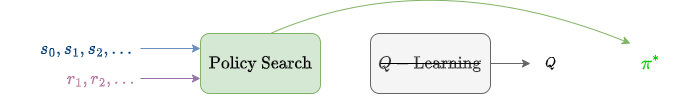
\includegraphics[width=110mm,scale=0.5]{images/rl_images/policy_search.png}
            \caption*{Not only do we ignore $T$ and $R$, but even $Q$.}
        \end{figure}

        Our strategy is to represent our policy as a \purp{function} with \gren{parameters} we can optimize.\\

        \begin{definition}
            In \vocab{policy search}, we represent our policy $\pi$ as a \textit{differentiable} \orgg{function} $f$, with \purp{parameters} $\theta$.

            \begin{itemize}
                \item This approach treats our policy like a \gren{hypothesis}.
            \end{itemize}

            \begin{equation*}
                \grn{\pi}\big(\red{s}\big) \;\;=\;\; f\big(\red{s}; \; \blu{\theta}\big) \;\;=\;\; \bro{a}
            \end{equation*}

            Using this approach, we can \orgg{optimize} our parameters $\theta$, to get the greatest average reward.

            \begin{itemize}
                \item We need our function to be differentiable, for the same reasons as we needed for \purp{gradient descent}.
            \end{itemize}
        \end{definition}

        One possible problem: often, we have a \purp{discrete} action space. Our output will be a category: \gren{not a continuous variable}.

        \begin{itemize}
            \item Discrete outputs aren't differentiable!
        \end{itemize}

        Our solution is the same as it was in classification: we use \purp{probabilities}.\\

        \begin{concept}
            Rather than outputting the chosen action, $a$, we output the \purp{probability} of that action.

            \begin{itemize}
                \item Because we chose our \brow{action} \gren{based on} our \redd{state}, it's a \vocab{conditional probability}:
            \end{itemize}

            \begin{equation*}
                f\Big( \red{s}, \bro{a}; \;\; \blu{\theta} \Big) \;\;=\;\; \given{\bro{a}}{\red{s}} 
                \;\;=\;\; 
                \text{Prob of choosing \brow{action $a$}, given \redd{state $s$}}
            \end{equation*}

            This allows us to output a \orgg{continuous} variable.
        \end{concept}

        Once we have our continuous function, we can use \vocab{gradient descent}.\\

        \begin{kequation}
            If $\theta$ is \gren{low-dimensional}, we can use \vocab{numerical gradient descent}/ascent to train our policy:

            \begin{itemize}
                \item Slightly \orgg{adjust} $\theta_i$ by $\eps$, see whether the \purp{total reward} $R$ is higher or lower: we approximate the derivative.

                    \begin{equation*}
                        \pderiv{R}{\theta_i} 
                        \;\;\approx\;\; 
                        \frac{\Delta R }{ \Delta \theta_i}
                        =
                        \frac{\pur{R}(\theta_i+\org{\eps})-\pur{R}(\theta_i)}{\org{\eps}} 
                    \end{equation*}
                \item Repeat for every $\theta_i$ term, to get a \gren{numerical gradient}.

                    \begin{equation*}
                        \nabla_\theta \pur{R}  = 
                        \begin{bmatrix}
                            \pderivslash{\pur{R}}{\theta_1} \\
                            \pderivslash{\pur{R}}{\theta_2} \\
                            \vdots \\
                            \pderivslash{\pur{R}}{\theta_n}
                        \end{bmatrix}
                    \end{equation*}

                \item Apply \vocab{gradient ascent} (we want to maximize $R$, rather than minimize $\loss$)

                    \begin{equation*}
                        \theta \;\;\Leftarrow\;\; \blu{\theta} \;+\; \red{\eta} \cdot \nabla_{\blu{\theta}}\pur{R} 
                    \end{equation*}

                
            \end{itemize}

            We could use \vocab{gradient descent} by choosing $\loss=-R$.

        \end{kequation}

        For problems with higher-dimensional $\theta$, this is often too slow/inefficient.

        \begin{itemize}
            \item Instead, we use other, more complex algorithms, like REINFORCE.
                \note{But these algorithms are often tricky.}
        \end{itemize}

        Policy search works best in those lower-dimensional cases.\\

        \begin{concept}
            \vocab{Policy search} works best when 

            \begin{itemize}
                \item The policy's \orgg{functional} form is known and \gren{simple}.
                \item Estimating the MDP would be \purp{difficult}.
            \end{itemize}
        \end{concept}



\pagebreak

\section{Model-based RL}

    Rather than try to directly compute $\pi$ or $Q$, we could also \textit{re-use} our previous techniques: we just need to compute $T$ and $R$.

    \begin{figure}[H]
        \centering
        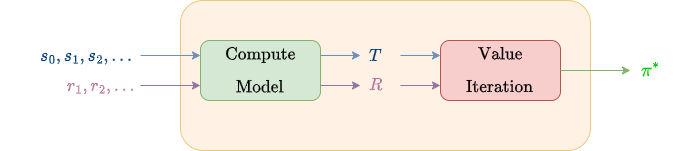
\includegraphics[width=90mm,scale=0.5]{images/rl_images/model_based.png}
        \caption*{Once we compute $T$ and $R$, we can do value iteration, like we did before.}
    \end{figure}

    \begin{notation}
        We want to \purp{approximate} $T$ and $R$.

        We'll represent these approximations as $\widehat{T}$ and $\widehat{R}$, respectively.
    \end{notation}

    \subsection{Computing $\widehat{T}$}

        To compute $\widehat{T}$, let's remind ourselves: what does $T$ represent?\\
            
        \begin{definition}
            \textit{Review from MDP Chapter, pt. 1:}
            
            The \vocab{transition function} $T$ gives the probability of 
    
            \begin{itemize}
                \item Entering state $\pur{s'}$,
                \item Given that we chose action $\bro{a}$ in state $\red{s}$
            \end{itemize}
    
            \begin{equation*}
                T(\red{s},\bro{a},\blu{s'}) \;\;=\;\; 
                \given{ \blu{S_t = s'}  }{\red{S_{t-1} = s},\quad \bro{A_t = a}}
            \end{equation*}
    
            After a transition, we will be in \orgg{exactly one} new state $s'$.
    
        \end{definition}
    
        So, we want to compute this probability. \\
    
        \begin{kequation}
            We can \purp{approximate} the probability of event $E$ happening, by \gren{counting} the number of times it does/doesn't occur:
            
            \begin{equation*}
                \prob{\pur{E}} \;\;=\;\; \frac{\text{Number of times } \pur{E} \text{ happens}}{\text{Total number of chances for $\pur{E}$ to happen}}
            \end{equation*}
    
            or,
    
            \begin{equation*}
                \prob{E} = \frac{\#E}{\#\text{Total events}}
            \end{equation*}
        \end{kequation}
    
        Let's apply this to our situation: first, our "total events".
    
        \begin{itemize}
            \item We're computing the probability, \purp{if} we chose action $\bro{a}$, in state $\red{s}$.
                \note{If we were in a \redd{different state}, or chose a \brow{different action}, then that doesn't affect the probability.}
    
                \begin{equation}
                    \#\text{Total events} = \#(\red{s},\bro{a})
                \end{equation}
    
            \item And we're looking for the chance that we \purp{enter state $s'$}.
    
                \begin{equation}
                    \#E = \#(\red{s},\bro{a},\blu{s'})
                \end{equation}
        \end{itemize}
    
        So, we get:
    
        \begin{equation}
            \overbrace{
            \qquad 
            \widehat{T}(\red{s},\bro{a},\blu{s'}) \;\;\approx\;\; \frac{\#(\red{s},\bro{a},\blu{s'})}{\#(\red{s},\bro{a})} 
            \qquad 
            }^{\text{Not our final equation}}
        \end{equation}

        But there's a \redd{problem} with this equation.




    \phantom{}

    \subsection{The Laplace Correction}

        In particular, we have \textit{two} problems with this equation.
    
        \begin{itemize}
            \item If we have \purp{no data}, what's our estimated probability? $0/0$.
            
                \begin{itemize}
                    \item This is \gren{nonsense}: we're dividing by zero.
                \end{itemize}
    
            \item If we have \purp{one data point}, and didn't get $E$, what is our probability? $0/1=0$.
    
                \begin{itemize}
                    \item If we have only one data point, why should we be so sure that $E$ \gren{never} happens?
                \end{itemize}
        \end{itemize}
    
        \begin{concept}
            The equation
    
            \begin{equation*}
                \prob{E} = \frac{\#E}{\#\text{Total events}}
            \end{equation*}
    
            Has two major flaws:
    
            \begin{itemize}
                \item It gives a \orgg{non-number} if we have no data.
    
                \item If we have \gren{no events} $E$, it says that there's a \purp{0\% chance} that $E$ will appear. Our model shouldn't be so confident.
            \end{itemize}
        \end{concept}
    
        \miniex Imagine you flipped a coin 3 times, and happened to get heads 3 times. This will happen $1/8$ of the time, on a fair coin.
    
        \begin{itemize}
            \item But our model has decided that there's a 0\% chance of ever getting tails.
        \end{itemize}
    
        Let's solve each of these problems:
    
        \begin{itemize}
            \item We don't want to \purp{divide by 0}. We need to add something to the \purp{bottom}.

            \item We don't want to give a \gren{0\% chance of $E$}, when we don't have enough data. We'll add something to the \gren{top}.
        \end{itemize}

        \begin{equation}
            \qquad 
            \widehat{T} (\red{s},\bro{a},\blu{s'})  \;\;=\;\;
            \frac{\#(\red{s},\bro{a},\blu{s'}) + b}{\#(\red{s},\bro{a}) + c} 
            \qquad 
        \end{equation}

        How do we decide these constants? Well, let's return to the situation where we have \redd{no data}.

        \begin{equation}
            \qquad 
            \widehat{T}(\red{s},\bro{a},\blu{s'}) \;\;=\;\;
            \frac{b}{c} 
            \qquad 
        \end{equation}

        We want $b/c$ to be our "\orgg{default}" assumption: what do we think are the odds of transitioning to state $\blu{s'}$, without any data?

        \begin{itemize}
            \item We have $\abs{\mathcal{S}}$ different states, that we could \gren{transition} to. 
            \item Without any data, we have no reason to prefer one state over another. So, we assume all states to be \purp{equally likely}.
        \end{itemize}

        If we split our probability evenly, we get:

        \begin{equation}
            \qquad 
            \widehat{T}(\red{s},\bro{a},\blu{s'}) \;\;=\;\;
            \frac{1}{\abs{\mathcal{S}}}
            \qquad 
        \end{equation}

        We have our \purp{correction terms}.\\

        \begin{definition}
            The \vocab{laplace correction} is an adjustment to our \purp{probability equation}, that solves the problems of 

            \begin{itemize}
                \item Dividing by 0
                \item Computing probability to be 0, with very low data
            \end{itemize}

            The solution is to set a \orgg{default} probability for an event: we split probability \gren{evenly} between all of our \gren{$N$ possible outcomes}.

            \begin{equation*}
                \given{E}{\text{No data}} \;\;=\;\; \frac{1}{N}
            \end{equation*}

            Applying this to our general equation, we get

            \begin{equation*}
                \prob{E} \;\;\approx\;\; \frac{\grn{1}\;+\;\#E}{\grn{N} \;+\; \#\text{Total}}
            \end{equation*}

            As we gather more data, this correction term gradually \orgg{vanishes}.
        \end{definition}

        \miniex Let's say we have \gren{5 possible outcomes}, and the odds of our event $E$ are 40\% (0.4).
            \note{And let's say our data exactly matches our probability, just to make things easier.}

        \begin{itemize}
            \item We'll compare the prediction for 5,50, and 500 data points.

            \begin{equation*}
                \frac{\grn{1}+2}{\grn{5}+5} = 0.3 \qquad \qquad 
                \frac{\grn{1}+20}{\grn{5}+50} \approx 0.381 \qquad \qquad
                \frac{\grn{1}+200}{\grn{5}+500} \approx 0.398
            \end{equation*}

            \item As we get more data, the laplace correction becomes less and less important.
        \end{itemize}

        

        Now, we can show our approximation for $T$.\\


        \begin{kequation}
            Our \vocab{approximation} for the transition function $T$ is given by the equation

            \begin{equation*}
                \widehat{T} (\red{s},\bro{a},\blu{s'})  \;\;=\;\;
                \frac{\#(\red{s},\bro{a},\blu{s'}) \;+\;\grn{1}}{\#(\red{s},\bro{a}) \;+\; \grn{\abs{\mathcal{S}}}} 
            \end{equation*}
        \end{kequation}




    \pagebreak

    \subsection{Computing $\widehat{R}$}

        Our reward function $R$, on the other hand, is much simpler to "approximate", because it's \orgg{deterministic}:

        \begin{itemize}
            \item The same state-action pair $(\red{s},\bro{a})$ will \purp{always give the same reward}.
            \item So, we don't have to approximate our reward: if we get our reward once, we know \gren{exactly} what it'll be.\\
        \end{itemize}

        \begin{kequation}
            Our "\vocab{approximation}" for the reward function $R$ comes directly from our observations:

            \begin{equation*}
                \widehat{R}(\red{s},\bro{a}) = \pur{r_t} \qquad \qquad 
                \text{if } \;\;\red{s_{t-1}=s}, \;\; \bro{a_t=a}
            \end{equation*}

            This isn't really an approximation: it gives our \gren{exact reward}.

            \begin{equation*}
                \widehat{R}(\red{s},\bro{a}) \;\;=\;\; 
                \pur{r_t}  \;\;=\;\; 
                R(\red{s},\bro{a})
            \end{equation*}
        \end{kequation}

        \subsecdiv

        In some situations, our reward might not be deterministic.

        \begin{itemize}
            \item In which case, we can compute the reward probability function, or the expected reward for our state-action pair.
        \end{itemize}




    \phantom{}

    \subsection{Solving our MDP}

        Once we've computed our approximations $\widehat{T}$ and $\widehat{R}$, we can now construct the "approximated MDP":

        \begin{equation}
            MDP \Big( \red{\mathcal{S}}, \bro{\mathcal{A}}, \grn{\widehat{T}}, \pur{\widehat{R}}, \blu{\gamma} \Big) 
        \end{equation}

        And we can just solve it like any other MDP, using a technique like \purp{value iteration}.\\

        \begin{definition}
            Our \vocab{model-based RL algorithm} has three basic parts: 
            
            \begin{itemize}
                \item Computing our model $ \Big( \red{\mathcal{S}}, \bro{\mathcal{A}}, \grn{\widehat{T}}, \pur{\widehat{R}}, \blu{\gamma} \Big) $.

                \begin{equation*}
                    \widehat{T} (\red{s},\bro{a},\blu{s'})  \;\;=\;\;
                    \frac{\#(\red{s},\bro{a},\blu{s'}) \;+\;\grn{1}}{\#(\red{s},\bro{a}) \;+\; \grn{\abs{\mathcal{S}}}} 
                \end{equation*}

                \begin{equation*}
                    \widehat{R}(\red{s},\bro{a}) = \pur{r_t} \qquad \qquad 
                    \text{if } \;\;\red{s_{t-1}=s}, \;\; \bro{a_t=a}
                \end{equation*}

                \phantom{}

                

                \item Using that model to do \orgg{value iteration}.

                    \begin{equation*}
                        \pur{Q\big(s,a \big)} \;\;=\;\; 
                                \widehat{R} \Big( s,a \Big)
                            \;\;+\;\;
                            \gamma
                            \pur{\sum_{s'}}  
                                \;\;
                                \widehat{T} \Big(          s,a,s' \Big)
                                \;\cdot\; 
                                \bro{ \max_{a'} \Big( \pur{Q\big(s',a' \big)} \Big)}
                    \end{equation*}

                \phantom{}

                

                \item Using $Q$-values to find the optimal policy.

                    \begin{equation*}
                        \grn{\pi^*}\big(\redd{s}\big) = 
                        \bro{\argmax{a}}{} \Big( 
                            Q\big(\red{s}, \bro{a} \big) 
                        \Big)
                    \end{equation*}
            \end{itemize}
        \end{definition}

        The approach requires us to approximate $T$ and $R$ for every possible combinations of input variables. 

        \begin{itemize}
            \item So we can't use it if our state space is too large.\\
        \end{itemize}

        \begin{concept}
            \vocab{Model-based RL algorithms} work best when we have a \purp{small, discrete} state space $\mathcal{S}$.

            \begin{itemize}
                \item They're difficult to generalize to \gren{large, or continuous} state spaces.
            \end{itemize}
        \end{concept}




    \pagebreak

\section{Bandit Problems}

    Here, we'll move away from our MDP framework.
    
    \begin{itemize}
        \item We'll consider a different kind of problem: one without \redd{states}.
    \end{itemize}



    \phantom{}

    \subsection{Slot machines}

        Here's our general idea: we have $k$ different \brow{choices} we can make. We want to \orgg{explore} each option, and figure out which one is the best.
            \note{No states here: just actions you can take.}
    
        \begin{itemize}
            \item This sounds simple: we just try each option \gren{once}, and pick the best one.
    
            \item But it's not so easy: each choice has a \purp{randomized} outcome. 
                \begin{itemize}
                    \item And each lever has different odds of giving you a particular reward.
                \end{itemize}
        \end{itemize}
    
    
        We can think of this problem like a "\vocab{slot machine}" with $k$ levers: each one has different odds of giving you a reward.
            \note{Slot machines have, in the past, been called "one-armed bandits", because they take your money. This is why we call these "bandit problems".}\\
    
        \begin{concept}
            In a \vocab{bandit problem}, you have a set of $k$ independent \brow{actions} you can choose from.
    
            \begin{itemize}
                \item Each action will give you a \orgg{randomized} reward.
            \end{itemize}
    
            You goal is to maximize the \purp{total rewards} you get (while training!)
        \end{concept}
    
        Again, note that \redd{states} have been completely removed from the problem.




    \phantom{}

    \subsection{Formalizing the Bandit Problem}

        We'll define each part of the bandit problem.

        \begin{itemize}
            \item First, we'll need our "options", or \brow{actions $\mathcal{A}$}.

            \item What are the possible \purp{rewards} we can get? That's our set \pur{$\mathcal{R}$}.

            \begin{equation*}
                \bro{a \in \mathcal{A}} \qquad \qquad 
                \pur{r \in \mathcal{R}}
            \end{equation*}

        \end{itemize}

        Finally, we need the \orgg{probability} of getting a reward, if we take an action. This is similar to the \gren{transition function} $T$: 

        

        \begin{itemize}
            \item Rather than returning our next state $\blu{s'}$, it instead gives us the \purp{odds} of ending up in state $\blu{s'}$.
                \note{\textit{If} we take \brow{action $a$} in \redd{state $s$}.}
        \end{itemize}

        In the same spirit, we'll have a function $R_p$, which gives us the \orgg{probability} of getting \purp{reward $r$}, from \brow{action $a$}.

        \begin{equation}
            R_p(\bro{a},\pur{r}) \;\;=\;\; \prob{\text{Getting \purp{reward $r$} from \brow{action $a$}}}
        \end{equation}

        Using conditional notation,

        \begin{equation}
            R_p(\bro{a},\pur{r}) \;\;=\;\; \given{ \pur{r} }{ \bro{a} }
        \end{equation}

        Based on our inputs and outputs, we can write this with \orgg{function notation}:
            \note{$R_p: ( \bro{\mathcal{A}} \cross \pur{\mathcal{R}} )
            \rightarrow \RR$, where $\RR$ are real numbers, is also acceptable.}

        \begin{equation}
            R_p: \Big( \bro{\mathcal{A}} \cross \pur{\mathcal{R}} \Big)
            \rightarrow \Big[ 0,1 \Big]
        \end{equation}

        These are the three parts of our bandit problem.\\

        \begin{definition}
            A \vocab{bandit problem} has three parts:

            \begin{itemize}
                \item A set of actions $\bro{\mathcal{A}}$

                \item A set of rewards $\pur{\mathcal{R}}$

                \item A \orgg{reward-probability} function 

                    \begin{equation*}
                        R_p: \Big( \bro{\mathcal{A}} \cross \pur{\mathcal{R}} \Big)
                        \rightarrow \Big[ 0,1 \Big]
                    \end{equation*}

                    That tells us the \orgg{chance} of getting reward $\pur{r}$, from action $\bro{a}$.
            \end{itemize}
        \end{definition}


        Bandit problems are very, very important to reinforcement learning, and computer science.

        \begin{itemize}
            \item But we won't go through solutions/theorems here.
        \end{itemize}



    \phantom{}

    \subsection{$k$-armed bandit problem}

        The simplest version of this problem is called the \vocab{$k$-armed bandit problem}:

        \begin{itemize}
            \item Every action ("arm") will either provide a reward ($r=1$) or not ($r=0$).
        \end{itemize}

        So, each action varies only by the \purp{chance} that you get a reward.
            \note{In other words, we don't have "different types" of rewards.}\\

        \begin{definition}
            The \vocab{$k$-armed bandit problem} is a simplified bandit problem, where

            \begin{itemize}
                \item You either get a simple \purp{reward}, or you get nothing: $\pur{\mathcal{R}} = \setty{0,1}$

                \item You have \brow{$k$ actions} to choose from: $\abs{\bro{\mathcal{A}}}=k$
            \end{itemize}
        \end{definition}



    \phantom{}

    \subsection{Exploration vs. Exploitation}

        In bandit problems, you have to balance \vocab{exploration vs. exploitation}:

        \begin{itemize}
            \item \purp{Exploration}: Do we want to improve our \orgg{estimate}, $\widehat{R}_p$? The better our estimate is, the more likely we are to make optimal choices, moving forward.

            \item \gren{Exploitation}: Do you want to maximize your rewards, \orgg{based on} $\widehat{R}_p$? You'll get more benefits short-term than if you keep exploring.
        \end{itemize}

        If you want to maximize your rewards, while still \orgg{learning}, you can't just explore, and you can't "exploit" blindly without data.

        There's lots of interesting details we'll skip here, but the basic idea is:\\

        \begin{concept}
            The longer your horizon $h$ (or the larger $\gamma$ is), the longer you should continue to \gren{explore}.

            \begin{itemize}
                \item The same amount of exploring takes up \gren{smaller fraction} of your time: so, it takes away \purp{less} of the exploitation reward.
            \end{itemize}
        \end{concept}


        \miniex Consider a simplified version: you have \orgg{$h$ turns} to play.
        
        You spend $n$ turns "exploring", and then $h-n$ turns "exploiting". You get 0 reward for exploring.
            \note{This example uses a lot of huge simplifications. Let's say these as "average" benefits for exploring/exploiting.}

        \begin{itemize}
            \item You get \pur{\$10} for exploiting if you explored a \purp{little} ($n=3$)

            \item You get \grn{\$15} for exploiting if you explored \gren{a lot} ($n=10$)
        \end{itemize}

        If you have only a little time (\org{$h=15$}), it's not really worth it to explore more.

        \begin{equation}
            \overbrace{(\org{15}-3) \cdot \pur{10} = 120 
            }^{\text{More time to exploit}}
            \qquad \qquad 
            \overbrace{
            (\org{15}-10) \cdot \grn{15} = 75
            }^{\text{More reward for exploiting}}
        \end{equation}

        If you have plenty of time (\org{$h=100$}), it's definitely worth it.

        \begin{equation}
            (\org{100}-3) \cdot \pur{10} = 970 \qquad \qquad (\orgg{100}-10) \cdot \grn{15} = 1350
        \end{equation}
        
        

        Of course, this exploration/exploitation process is fairly sensitive to "luck": whether we get better or worse outcomes than the average.
            \note{Which can happen very easily, with small sample sizes. 
            
            \phantom{}
            
            The longer we can train, the more likely we are to be near the true average.}\\
        

        \begin{concept}
            "\purp{Bad luck}" (getting low rewards for a valuable lever) is often more harmful than "\gren{good luck}" (getting high rewards for a bad lever):

            \begin{itemize}
                \item If you get bad luck, you're \purp{less likely} to keep trying that lever: you \orgg{won't find out} it's a good lever.
    
                \item If you get good luck, you'll probably \gren{keep trying} that (seemingly profitable) lever: you'll get \orgg{lots of data} to learn that it isn't as good as you thought.
            \end{itemize}

            
        \end{concept}




    \phantom{}
    

    \subsection{Contextual Bandit Problems}

        Our typical bandit problems lack the concept of a "\redd{state}". However, if we \textit{do} need states, we can use a \textit{contextual bandit problem}:\\

        \begin{definition}
            In a \vocab{contextual bandit problem}, we re-introduce \redd{states $\mathcal{S}$}.

            \begin{itemize}
                \item Each state $\red{s}$ has its own bandit problem.
            \end{itemize}
        \end{definition}

    
    


\pagebreak

\section{Terms}

    \begin{itemize}
        \item MDP (Review)
        \item Value function (Review)
        \item $Q$-value function (Review)
        \item Reinforcement Learning
        \item Learner
        \item Environment
        \item Supervised Learning (Review)
        \item Unsupervised Learning (Review)
        \item Model-based RL
        \item Model-free RL
        \item $Q$-learning
        \item Value iteration (Review)
        \item Learning rate $\alpha$
        \item $\epsilon$-greedy strategy
        \item Exploration vs. Exploitation
        \item Tabular $Q$-learning
        \item Deep $Q$-learning
        \item Temporally Correlated
        \item Catastrophic forgetting
        \item Experience Replay
        \item Replay Buffer
        \item Sliding Window
        \item Fitted $Q$-learning
        \item Policy search
        \item Conditional Probability (Review)
        \item Numerical Gradient Descent
        \item $\widehat{T}$
        \item $\widehat{R}$
        \item Laplace Correction
        \item Bandit Problem
        \item Reward-probability function $R_p$
        \item $k$-armed bandit problem
        \item Contextual Bandit Problem
    \end{itemize}

        

    

    
    

    

    

    

        

    



        

        
